%---------
% PREAMBLE
%---------
\documentclass[man]{apa7} % Layout standard

% PACKAGES
\usepackage[american]{babel} % Multilingual support for Plain TEX or LATEX
\usepackage{csquotes} %  Inline and display quotations
\usepackage[style=apa,sortcites=true,sorting=nyt,backend=biber]{biblatex}
\usepackage{caption} 

% PACKAGES - Figures
\usepackage{subcaption} % Allow for subfigures

% PACKAGES - Tables
\usepackage{threeparttable}
\usepackage{multirow}

% PACKAGES - Math
\usepackage{amsmath}
\usepackage{amssymb}
\usepackage{amsfonts}
\usepackage{mathabx}
\usepackage{mathtools}
\usepackage{bbm}

% PACKAGES - Page orientation
\usepackage{rotating,threeparttable,booktabs,caption,dcolumn}

\DeclareLanguageMapping{american}{american-apa}

% REFERENCES
\addbibresource{references.bib}

%-----------
% TITLE PAGE  
%-----------
\title{Time Aggregation and Missing Time Frames in Causal Research With Panel Data}
\shorttitle{Time Aggregation in Causal Research}

\authorsnames[1, 2, 1]{Jeroen D. Mulder, Manuel C. Voelkle, and Ellen L. Hamaker}
\authorsaffiliations{{Universiteit Utrecht, Utrecht, the Netherlands}, {Humboldt-Universität, Berlin, Germany}}

\leftheader{Mulder, Voelkle, Hamaker}

\abstract{A common goal in psychological and behavioral research is the study of causal mechanisms underlying a particular process of interest. These research questions are commonly investigated using panel data at relatively large time intervals of months or years and with measurements referring to the past week, month, or year. In this article, we investigate to what extend panel data can be used to study a causal mechanism when the causal process is assumed to play out at a (much) finer time scale than that of the panel data. Specifically, we used simulations to study the impact of time-aggregation and systematic (under)sampling on the ability of popular dynamic models to approximate the instantaneous effect of a time-varying exposure on a time-varying outcome in three different scenarios. The results illustrate how time-aggregation and systematic (under)sampling can lead to severe over- and underestimation of the causal effect, implying that wrong (and potentially harmful) conclusions can be draw. We discuss the implications of these findings for applied researchers, and describe how asking a different kind of causal question can help applied researchers to think about the role of time in their causal research.}

\keywords{dynamic models, time-aggregation, time scales, causal research, systematic (under)sampling}

\authornote{\addORCIDlink{Jeroen D. Mulder}{0000-0002-5553-0856}\\
   \addORCIDlink{Manuel C. Voelkle}{0000-0001-5576-8103}\\
   Jeroen D. Mulder and Ellen L. Hamaker are supported by Stress in Action (SiA). SiA is funded through the Gravitation Program of the Dutch Research Council and the Dutch Ministry of Education, Culture and Science (NWO grant number 024.005.010). Manuel C. Voelkle is in parts funded by the Deutsche Forschungsgemeinschaft (DFG, German Research Foundation) – 523691032. 
}

\begin{document}
\maketitle

%-----------
% MANUSCRIPT  
%-----------

\section{1. Introduction}
The analysis of panel data, in which the same people are repeatedly measured on the same variables, is wide-spread in psychology and related disciplines to investigate causal relationships between variables. These causal interpretations are sometimes explicit, but are typically left implicit through the use of specific language or suggestions for interventions based on analysis results \parencite{asendorpf_modeling_2021, grosz_taboo_2020, hamaker_description_2020}. To identify causal effects from data, it is critical that the research question and the research design are aligned in a temporal sense. For example, a typical research question in psychology may be about the effect of social media use on stress levels, or, phrased alternatively, understanding the causal mechanism underlying the relationship between social media use and stress. These kinds of questions are commonly answered with panel data that are characterized by repeated measures at monthly or yearly intervals. However, from a methodological perspective one may wonder if a research question about an ``underlying causal mechanism'' is a sensible question to ask when analyzing panel data and when the causal process between social media use and stress is believed to operate at a much finer grained time-scale \parencite[e.g., within-day or day-to-day;][]{collins_effect_2002}. This is also a concern that has been discussed in prior methodological studies, for example, in literature on continuous-time modeling \parencites[cf.][]{voelkle_sem_2012, voelkle_role_2018, batra_consequences_2023}, theory formation \parencite{mitchell_building_2001}, and study design \parencites[cf.][]{collins_effect_2002, collins_analysis_2006, hamaker_within-between_2023}. In this article we expand the discussion of this concern, focusing on misalignment of the temporal characteristics of a causal mechanism of interest and the timescale of measurements, and the consequences thereof for the identification and estimation of a causal effect from observed longitudinal data.

We concentrate on two common measurement-related features in panel data that can lead to temporal misalignment, namely \textit{time-aggregation} of variables and \textit{low process coverage} due to systematic (under)sampling. Time-aggregation refers to measurements that pertain to an average level of a construct across a particular time-period, rather than the level of the construct at the moment of measurement \parencite{petkovic_aggregation_2009}. For example, in psychological research, it is relatively common to ask participants of panel studies to provide aggregate scores for themselves, by using questions that refer to participants' average levels of anxiety or self-esteem across \textit{the past week} or \textit{the past month}, rather than their levels of anxiety or self-esteem \textit{right now}. Furthermore, the concept of low process coverage refers to the situation where the combination of systematic (under)sampling over time (i.e., taking measurements at regular intervals that are too long in relation to the timescale at which the process operates) and time-aggregation of measurements only captures a small part of a continuous process. For example, \textcite{hamaker_within-between_2023} describes how the combination of biannual measurement occasions with measurements referring to the past week, implies that less then 1\% of an ongoing process is actually covered by measurements. Both of these features can negatively impact a researcher's ability to identify and estimate from the data effects of causal mechanisms at finer time scales. The current paper studies this impact in the context of causal inference using panel data, and demonstrates it in multiple simulation scenarios. 

This paper is organized as follows. To aid explanation of time-aggregation and low process coverage, we first introduce these concepts in the context of single-subject (i.e., $N = 1$) research with many repeated measures. Section 2 provides an overview of early analytical work on the impact of time-aggregation of variables on the performance of dynamic models for $N = 1$ data. It also introduces the impact of low process coverage from a causal inference perspective. In Section 3, we present a simulation study to extend previous analytical work. These simulations focus on (a) the combined influence of time-aggregation and low process coverage for $N = 1$ data; (b) time-aggregation and low process coverage in $N = 1$ data in the presence of a time-varying confounder; and (c) time aggregation and low process coverage for \textit{panel data} and in the presence of a time-varying confounder. Section 4 discusses the implications of the results for current causal research using panel data, and suggests future directions for addressing some of the concerns raised. Throughout, we use a running example that is motivated by panel research concerning the impact of social media use on anxiety in early-adolescents. Specifically, we take inspiration from the Longitudinal Internet studies for the Social Sciences (LISS) panel, which consists of a random sample of Dutch households representative of the Dutch-speaking population in the Netherlands, and which contains annual measurements covering a large variety of domains \parencite{das_true_2018}. In the LISS panel, anxiety was measured with the statement ``This past month... I felt very anxious.'', with participants having to indicate which answer best described them on a scale from ``1 = never'' to ``6 = continuously''. Social media usage was measured by asking participants how many hours per week \textit{on average} they spend on social media, but without providing an explicit time frame (i.e., whether the average refers to the past week, past month, past year, a randomly chosen week in the past year, etc.). 

\section{2. Background}
Much of the early work on the impact of time-aggregation of variables and systematic (under)sampling comes from the econometric literature, and was driven by the time-aggregation of economic variables before analyses. For instance, the aggregation of \textit{momentary} stock prices to \textit{day-averages}, or the transformation of \textit{monthly} gross domestic product figures to \textit{quarterly} aggregates \parencite{mundlak_aggregation_1961, telser_discrete_1967}. This work focuses specifically on dynamic models for time series data, such as the lag-1 autoregressive model, the AR(1), and its extension with a time-varying covariate $X$, the ARX(1). Because early analytical work on time-aggregation concerns time series data, and because dynamic models form the backbone of many of the current statistical models used to analyze panel data in psychology \parencite[e.g., the class of cross-lagged panel models;][]{usami_unified_2019}, we introduce these dynamic models first in Section 2.1. In Section 2.2, we discuss the implications of time-aggregation for the AR(1) model. Section 2.3 introduces the issues of low process coverage from a causal inference perspective. 

\subsection{2.1 Dynamic Models}
Let the continuous variable $t$ represent time, and the variable $k$ denote a measurement occasion at a particular point in time. The AR(1) model describes the relationship between a variable at occasion $k$, $Y_{k}$, and the values of that same variable at the previous occasion, $Y_{k - 1}$. It can be expressed as
\begin{equation} \label{eq:AR1}
    Y_{k} = \phi Y_{k - 1} + \epsilon_{Y,k}. 
\end{equation}
$\phi$ represents the lag-1 autoregressive coefficient of the regression of $Y_{k}$ on $Y_{k - 1}$. Since we only consider AR(1) processes in the present manuscript, we refrain from adding the index $_{k - 1}$ to $\phi$ to simplify the notation. $\epsilon_{Y,k}$ is a residual for the outcome $Y$ at occasion $k$ that is typically assumed to be mean-zero normally distributed with variance $\sigma_{\epsilon_{Y}}^{2}$. Equation~\ref{eq:AR1} does not include an intercept term, hence we assume the mean of $Y_{k}$ to be zero. 

To investigate relationships between variables, the AR(1) model can be extended with an exogenous time-varying predictor $X$. Given that causes need time to exert an effect, often a lagged version of $X$ is added as a predictor to the model, resulting in 
\begin{equation}
    Y_{k} = \phi Y_{k - 1} + \beta_{k - 1} X_{k - 1} + \epsilon_{Y,k}. 
\end{equation}
Here, $\beta_{k - 1}$ represents the lag-1 effect from $X$ to $Y$. However, it has been argued that when the time interval is large and the causal effect of $X$ under study is relatively rapid, that lagged effects of $X$ should not be added \parencite{mundlak_aggregation_1961}. Instead, lag-0 effects could be added to the model, resulting in the ARX(1) model. It is given by
\begin{equation} \label{eq:ARX1}
    Y_{k} = \phi Y_{k - 1} + \beta_{k} X_{k} + \epsilon_{Y,k}, 
\end{equation}
where $\beta_{k}$ now represents the lag-0 (rapid) effect of the time-dependent predictor on the outcome. Similar discussions about modeling instantaneous effects have taken place in the context of panel data analysis \parencite{greenberg_panel_1979, greenberg_equilibrium_1982}, and more recently by \textcite{muthen_can_2024} in the context of cross-lagged panel modeling in the structural equation modeling (SEM) framework. 

\subsection{2.2 Time-Aggregation}
There exist various forms of time-aggregation, also referred to as \textit{aggregation schemes}. In this paper, we discuss time-aggregation that concerns taking the mean across a particular period of time, as this is a relatively common aggregation-scheme in psychological measurements. To this end, we introduce some additional notation below. Let $m$ be the number of time periods that we aggregate over, and suppose that in our running example the anxiety-process operates on a day-to-day basis. Further suppose for simplicity's sake that each month consists of four weeks, and thus 28 days. As mentioned in the introduction, anxiety is measured in the LISS panel data with the question ``This past month... I felt very anxious.'', implying that participants are expected to average their daily anxiety levels over the past $m = 28$ periods (days). To distinguish between measurements of the disaggregated process ($m = 1$) and aggregated measurements ($m > 1$), we add the subscript $_{(m)}$ to variable names, such that $Y_{k_{(m)}}$ represents the outcome $Y$ at measurement $k$ aggregated over $m$ occasions: Disaggregated measurements are then denoted by $Y_{k_{(1)}}$ and 28-day-aggregated measurements by $Y_{k_{(28)}}$. Furthermore, we focus on aggregate measurements that are ``proper'', that is, aggregate measurements are measured back-to-back and do not overlap. For example, with anxiety measured as 28-day-averages, we would only include the aggregates of day 1 to day 28, day 29 to day 56, day 57 to day 84, and so on in our analysis, which are then denoted as $Y_{1_{(28)}}$, $Y_{2_{(28)}}$, and $Y_{3_{(28)}}$, respectively. Intermediate overlapping frames, such as aggregates from day 1 to day 28, day 2 to day 29, day 3 to day 30, are not considered. Figure~\ref{fig:notation} illustrates this notation for aggregation over $m = 2, 3$ periods. 

\begin{figure}
    \centering
    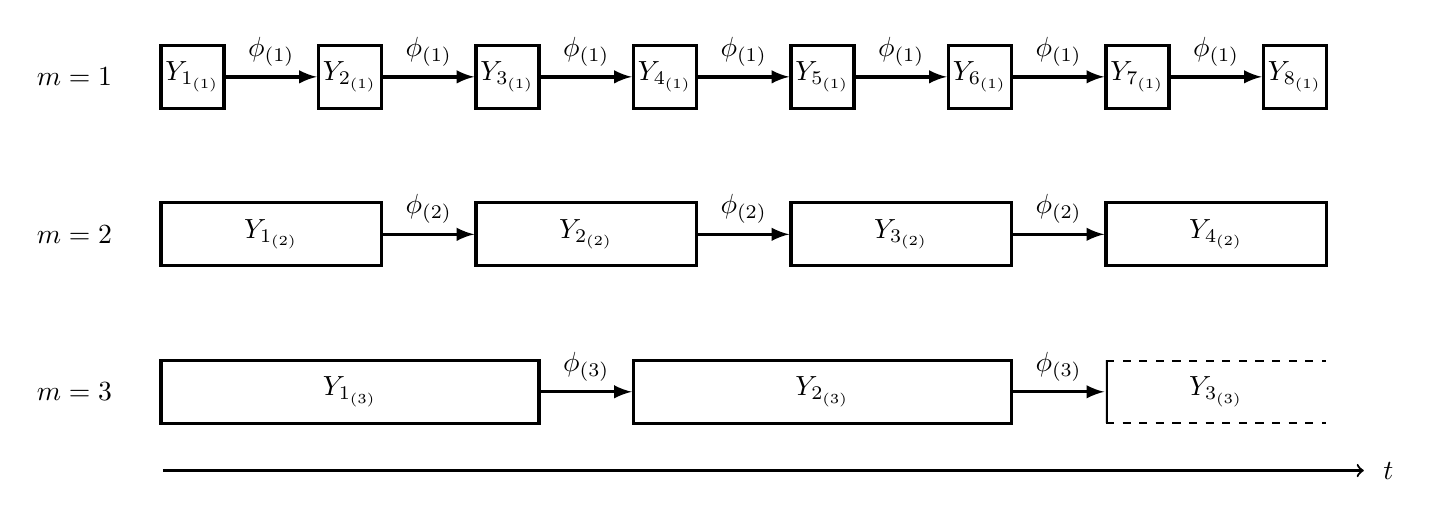
\begin{tikzpicture}[auto, scale = 0.5,
        time/.style={rectangle, inner sep=0pt, minimum size=8mm, align=center},
        manifest/.style={rectangle,draw,very thick,inner sep=0pt,minimum width=8mm,minimum height=8mm},
        paths/.style={->, very thick, -latex},
        openbox/.style={
            rectangle, very thick,
            minimum width=28mm, minimum height=8mm,
            path picture={
                \draw[dashed] (path picture bounding box.north west) -- (path picture bounding box.north east); % top line
                \draw[dashed] (path picture bounding box.south west) -- (path picture bounding box.south east); % bottom line
                \draw (path picture bounding box.north west) -- (path picture bounding box.south west); % left side
            }
        },
        double/.style={very thick, -latex}
    ]
    
        % Nodes
        \node[manifest] (y11) at (0,0) {$Y_{1_{(1)}}$};
        \node[manifest, right of = y11, xshift = 1cm] (y21) {$Y_{2_{(1)}}$};
        \node[manifest, right of = y21, xshift = 1cm] (y31) {$Y_{3_{(1)}}$};
        \node[manifest, right of = y31, xshift = 1cm] (y41) {$Y_{4_{(1)}}$};
        \node[manifest, right of = y41, xshift = 1cm] (y51) {$Y_{5_{(1)}}$};
        \node[manifest, right of = y51, xshift = 1cm] (y61) {$Y_{6_{(1)}}$}; 
        \node[manifest, right of = y61, xshift = 1cm] (y71) {$Y_{7_{(1)}}$};
        \node[manifest, right of = y71, xshift = 1cm] (y81) {$Y_{8_{(1)}}$}; 
                
        \node[manifest, below of = y11, yshift = -1cm, xshift = 1cm, minimum width=28mm] (y12) {$Y_{1_{(2)}}$};
        \node[manifest, below of = y31, yshift = -1cm, xshift = 1cm, minimum width = 28mm] (y22) {$Y_{2_{(2)}}$};
        \node[manifest, below of = y51, yshift = -1cm, xshift = 1cm, minimum width = 28mm] (y32) {$Y_{3_{(2)}}$};
        \node[manifest, below of = y71, yshift = -1cm, xshift = 1cm, minimum width = 28mm] (y42) {$Y_{4_{(2)}}$};
    
        \node[manifest, below of = y21, yshift = -3cm, minimum width = 48mm] (y13) {$Y_{1_{(3)}}$};
        \node[manifest, below of = y51, yshift = -3cm, minimum width = 48mm] (y23) {$Y_{2_{(3)}}$};
        \node[openbox, below of = y71, yshift = -3cm, xshift = 1cm] (y33) {$Y_{3_{(3)}}$};
    
        \node[left of = y11, xshift = -0.5cm] {$m = 1$};
        \node[left of = y12, xshift = -1.5cm] {$m = 2$};
        \node[left of = y13, xshift = -2.5cm] {$m = 3$};
    
        % Paths: Autoregressive effects                
        \draw[paths] (y11) -- (y21) node[midway, above] {$\phi_{(1)}$};
        \draw[paths] (y21) -- (y31) node[midway, above] {$\phi_{(1)}$};
        \draw[paths] (y31) -- (y41) node[midway, above] {$\phi_{(1)}$};
        \draw[paths] (y41) -- (y51) node[midway, above] {$\phi_{(1)}$};
        \draw[paths] (y51) -- (y61) node[midway, above] {$\phi_{(1)}$};
        \draw[paths] (y61) -- (y71) node[midway, above] {$\phi_{(1)}$};
        \draw[paths] (y71) -- (y81) node[midway, above] {$\phi_{(1)}$};
    
        \draw[paths] (y12) -- (y22) node[midway, above] {$\phi_{(2)}$};
        \draw[paths] (y22) -- (y32) node[midway, above] {$\phi_{(2)}$};
        \draw[paths] (y32) -- (y42) node[midway, above] {$\phi_{(2)}$};
    
        \draw[paths] (y13) -- (y23) node[midway, above] {$\phi_{(3)}$};
        \draw[paths] (y23) -- (y33) node[midway, above] {$\phi_{(3)}$};
                
        % Time line                
        \node (timeline-start) [below of = y13, xshift = -2.5cm] {};
        \node (timeline-end) [below of = y33, xshift = 2cm] {};
         
        \draw[->, thick] (timeline-start) -- (timeline-end) node[midway, above] {};
        \node at (timeline-end) [right] {$t$};  % Add letter t to the right of the timeline
    
    \end{tikzpicture}
    \vspace{1cm}
    \caption{A visualization of a disaggregated ($m = 1$) lag-1 autoregressive processes over time $t$, and $m = 2$ and $m = 3$ aggregated measurements thereof. $Y_{k_{(m)}}$ represents an outcome $Y$ at measurement occasion $k$ when mean-aggregating over $m$ periods. For example, $Y_{3_{(2)}}$ is the third measurement when aggregating over $m = 2$ periods, and is computed by taking the mean of $Y_{5_{(1)}}$ and $Y_{6_{(1)}}$ from the disaggregated process. Each aggregation scheme is characterized by its own set of parameters, which we distinguish by concatenating the subscript ${(m)}$ to the parameter. That is, the disaggregated process has an autoregressive effect $\phi_{(1)}$, whereas the autoregressive parameters of the $m = 2$ and $m = 3$ aggregated measurements are $\phi_{(2)}$ and $\phi_{(3)}$, respectively. The dotted box of $Y_{3_{(3)}}$ signals that this aggregate also includes $Y_{9_{(1)}}$, not displayed in the Figure.}
    \label{fig:notation}
\end{figure}

For this aggregation scheme, it is interesting to compare the parameter coefficients of dynamic models based on aggregated data to parameter coefficients of the model that generated the disaggregated data, that is, the \textit{data generating mechanism}. To distinguishing between the parameters of a data generating mechanism (where $m = 1$) and those from estimation models based on aggregated data ($m > 2$), we concatenate the subscript ${(m)}$ to parameter coefficients. One potentially interesting hypothesis is that lagged parameters for various levels of $m$ are related to each other similar to how lagged parameters across different time intervals are related to each other. For example, for a disaggregated AR(1) model, it is well-known that a lag-2 autoregressive effect (i.e., skipping every other day of measurement such that the autoregressive effect refers to an effect across two periods) can be expressed as the lag-1 autoregresssive effect to the power two, that is $\phi_{(1)}^{2}$. More generally, in a disaggregated AR(1) model, the lag-$d$ autoregressive effect is expressed as $\phi_{(1)}^{d}$. 

\textcite{ironmonger_note_1959, nerlove_estimation_1959, telser_discrete_1967} investigate if a similar relationship exists between parameters from AR(1) models based on data with different levels of aggregation. They compare the autoregressive parameter $\phi_{(1)}$ from the data generating AR(1) model, to the autoregressive parameter from an AR(1) model that is fitted on the aggregated data. We express the AR(1) model for the aggregated data as
\begin{equation} \label{eq:AR1-aggregated}
    Y_{k_{(m)}} = \phi_{(m)} Y_{k_{(m)} - 1} + \epsilon_{Y,k_{(m)}},
\end{equation} 
where $\phi_{(m)}$ represents the autoregressive parameter as estimated using data that were aggregated across $m$ occasions. Of interest is whether $\phi_{(m)}$ is related to $\phi_{(1)}$, by taking $\phi_{(1)}$ to the power $m$, that is $\phi_{(1)}^{m}$. However, \textcite{ironmonger_note_1959, nerlove_estimation_1959, telser_discrete_1967} found that $\phi_{(m)}$ and $\phi_{(1)}^{m}$ are generally not equivalent. The problem is that the act of aggregation creates a particular structure in the data---specifically, a first-order moving average structure---at the $m = 1$ level. However, in proper aggregated data (where $m > 1$), information about this structure at the $m = 1$ level is not present. Therefore, models for aggregated data such as Equation~\ref{eq:AR1-aggregated} cannot correctly model all the structure in the data (i.e., the model is misspecified), and the autoregressive parameter for the aggregated process $\phi_{(m)}$ cannot simply be expressed as $\phi_{(1)}^{m}$. For this reason, \textcite{amemiya_effect_1972} argue that the dynamics of an aggregated process are qualitatively different from those of a disaggregated process, even though the aggregated measurements are created from the disaggregated process. 

To better understand the relationship between $\phi_{(m)}$ (for $m > 1$) and $\phi_{(1)}$, \textcite{hickman_effects_1972} express the OLS-estimate of $\phi_{(m)}$ as a function of $\phi_{(1)}$. They show that for a covariance stationary process (i.e., when $|\phi_{(1)}| < 1$ and with constant variance and covariance over time), $\phi_{(m)}$ is larger than $\phi_{(1)}^{m}$. \textcite{hickman_effects_1972} also generalize their analysis to more complicated models such as the ARX(1), comparing both the disaggregated autoregressive parameter $\phi_{(1)}$ and time-dependent effect of $X$, $\beta_{(1)}$, with their aggregated counterparts $\phi_{(m)}$ and $\beta_{(m)}$. While they are able to compute the probability limit of the coefficients of the aggregated ARX(1) model as a function of coefficients of the data generating mechanism, they note that ``This relationship is so complicated that no general tendencies can be observed until simplifying approximations are made'' \parencite[][p. 689]{amemiya_effect_1972}, and resort to simulations. In Section 3, we similarly rely on simulations to study the impact of time-aggregation and low process coverage in three different scenarios. 

\subsection{2.3 Process Coverage} 
In addition to time-aggregation of variables, panel data are also commonly characterized by repeated measurements of a process of interest at relatively large intervals; the process in between subsequent discrete time points remains unobserved. A critical issue here is the decision of how much time to allow for between measurements occasions, as the parameter estimates from typical discrete-time statistical models are dependent on the chosen time-interval \parencite{gollob_taking_1987}. That is, when using the LISS panel to regress anxiety levels on previous anxiety levels and social media use, the resulting estimates of autoregressive and cross-lagged effects refer to effects that take place over one year; if measurements had instead been taken every six months, analyses would have resulted in different autoregressive and cross-lagged effects even when the underlying causal process remains unchanged. The time interval between measurements in combination with the time-aggregation of those measurements determines the degree to which a process is actually captured (i.e., the process coverage) and how much remains unobserved \parencite{hamaker_within-between_2023}.  

In the context of panel data, measurements are typically taken at monthly or yearly intervals, but it is not unreasonable to assume many psychological processes are actually occurring at a finer timescale \parencite{dormann_optimal_2015, collins_effect_2002}. Therefore, it is of interest to study how parameters from dynamic models based on panel data are related to the parameters that govern a data generating mechanism that is theorized to occur at a finer timescale. As explained in Section 2.2, in a disaggregated AR(1) model, the autoregressive effect across $d$ periods is a function of the lag-1 autoregressive effect given by $\phi_{(1)}^{d}$. This logic similarly applies to aggregated data ($m > 1$), where the autoregressive relationship $\phi_{(m)}$ across every second measurement occasion is $\phi_{(m)}^{d}$. This implies that the autoregressive parameter of a day-to-day process would approach zero as the time interval between repeated measurements increases (e.g., to months or years). For ARX(1) models, the instantaneous effect of time-dependent exposures $\beta_{0_{(m)}}$ is independent of the time-interval between repeated measures; the autoregressive parameter of the ARX(1) model has the same dependency on the time-interval as the the autoregressive parameter in the AR(1) model \parencite{van_montfort_understanding_2018}. For dynamic models with multiple variables and higher-order effects, the relationship between parameters at varying time lags is more complex due to interacting direct and indirect effects, but is well-understood and described in the continuous-time literature \parencite[the interested reader is referred to][]{oud_sem_2018, van_montfort_continuous_2018}. 

Although the the relationship between parameters based on data at various time intervals is well-studied for dynamic processes, without additional assumptions, the unobserved part of the process in between measurement occasions poses a challenge from a causal inference perspective. Unbiased estimation of causal effects assumes that all confounders have been measured such that they can be adjusted for in a statistical analysis. However, suppose that two processes, such as anxiety levels and social media use, vary and interact with each other in discrete-time every day. This is illustrated in Figure~\ref{fig:DAG_ARX1_missingFrames_DGM} using a directed acyclic graph (DAG), which is a graphical representation of a causal process. In this DAG, and under a sampling scheme that takes measurement every other day, $X_{k_{(1)}}$ and $Y_{k_{(1)}}$ are social media use and anxiety levels on day 1, $X_{k_{(1)} + \frac{1}{2}}$ and $Y_{k_{(1)} + \frac{1}{2}}$ are social media use and anxiety levels on day 2, $X_{k_{(1)} + 1}$ and $Y_{k_{(1)} + 1}$ are social media use and anxiety levels on day 3, etc. The arrows represent causal effects between variables. Suppose further that our interest is in the within-day effect of social media use on stress $\beta_{0_{(1)}}$. To estimate the effect $\beta_{0_{(1)}}$ at occasion $k_{(1)} + 1$, we would need to adjust for social media use the previous day $X_{k_{(1)} + \frac{1}{2}}$, as this acts as a confounder for the direct relationship $X_{k_{(1)} + 1} \rightarrow Y_{k_{(1)} + 1}$. However, under a sampling scheme that takes measurements only every other day, social media use and anxiety levels for non-integer $k$-occasions (i.e., days 2, 4, etc.) remain unobserved. That is, researchers would only have the variables in Figure~\ref{fig:DAG_ARX1_missingFrames_observed} available to them. Therefore it is not possible to control for $X_{k_{(1)} + \frac{1}{2}}$ in an analysis model. In other words, the causal effect $\beta_{0_{(1)}}$ is unidentified in the data of Figure~\ref{fig:DAG_ARX1_missingFrames_observed}. 

\begin{figure}
    \centering
    \begin{subfigure}{\textwidth}
        \centering
        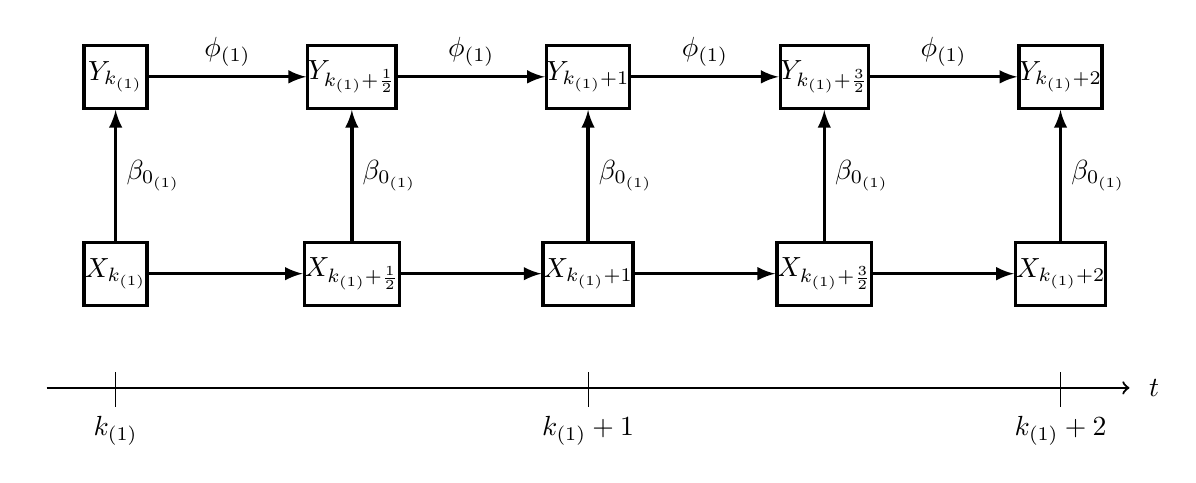
\begin{tikzpicture}[auto, scale = 0.5,
            time/.style={rectangle, inner sep=0pt, minimum size=8mm, align=center},
            manifest/.style={rectangle,draw,very thick,inner sep=0pt,minimum width=8mm,minimum height=8mm},
            paths/.style={->, very thick, -latex},
            double/.style={very thick, -latex}
        ]
            % Nodes
            \node[manifest] (y0) at (0,0) {$Y_{k_{(1)}}$};
            \node[manifest, right of = y0, xshift = 2cm] (y1) {$Y_{k_{(1)} + \frac{1}{2}}$};
            \node[manifest, right of = y1, xshift = 2cm] (y2) {$Y_{k_{(1)} + 1}$};
            \node[manifest, right of = y2, xshift = 2cm] (y3) {$Y_{k_{(1)} + \frac{3}{2}}$};
            \node[manifest, right of = y3, xshift = 2cm] (y4) {$Y_{k_{(1)} + 2}$};
                    
            \node[manifest, below of = y0, yshift = -1.5cm] (x0) {$X_{k_{(1)}}$};
            \node[manifest, below of = y1, yshift = -1.5cm] (x1) {$X_{k_{(1)} + \frac{1}{2}}$};
            \node[manifest, below of = y2, yshift = -1.5cm] (x2) {$X_{k_{(1)} + 1}$};
            \node[manifest, below of = y3, yshift = -1.5cm] (x3) {$X_{k_{(1)} + \frac{3}{2}}$};
            \node[manifest, below of = y4, yshift = -1.5cm] (x4) {$X_{k_{(1)} + 2}$};

            % Paths: Time-dependent effects
            \draw[paths] (x0) -- (y0) node[midway, right] {$\beta_{0_{(1)}}$};
            \draw[paths] (x1) -- (y1) node[midway, right] {$\beta_{0_{(1)}}$};
            \draw[paths] (x2) -- (y2) node[midway, right] {$\beta_{0_{(1)}}$};
            \draw[paths] (x3) -- (y3) node[midway, right] {$\beta_{0_{(1)}}$};
            \draw[paths] (x4) -- (y4) node[midway, right] {$\beta_{0_{(1)}}$};

            % Paths: Autoregressive effects
            \draw[paths] (x0) -- (x1);
            \draw[paths] (x1) -- (x2);
            \draw[paths] (x2) -- (x3);
            \draw[paths] (x3) -- (x4);
                    
            \draw[paths] (y0) -- (y1) node[midway, above] {$\phi_{(1)}$};
            \draw[paths] (y1) -- (y2) node[midway, above] {$\phi_{(1)}$};
            \draw[paths] (y2) -- (y3) node[midway, above] {$\phi_{(1)}$};
            \draw[paths] (y3) -- (y4) node[midway, above] {$\phi_{(1)}$};
                    
            % Time line                
            \node (timeline-start) [below of = x0, yshift = -0.45cm, xshift = -1cm] {};
            \node (timeline-end) [below of = x4, yshift = -0.45cm, xshift = 1cm] {};
             
            \draw[->, thick] (timeline-start) -- (timeline-end);
            \node at (timeline-end) [right] {$t$};  % Add letter t to the right of the timeline

            % Add ticks and labels for the timeline relative to the diagram nodes
            \node (k1) [below of = x0, yshift = -1cm] {$k_{(1)}$};
            \node (k2) [below of = x2, yshift = -1cm] {$k_{(1)} + 1$};
            \node (k3) [below of = x4, yshift = -1cm] {$k_{(1)} + 2$}; 
                
            \foreach \tick in {k1, k2, k3} {
                \draw (\tick) -- ++(0,1.5); 
            }
        \end{tikzpicture}
        \caption{A directed acyclical graph representing the causal dependencies between social media use $X$ and $Y$ anxiety over time.}
        \label{fig:DAG_ARX1_missingFrames_DGM}
    \end{subfigure}
    \vspace{1cm}
    \begin{subfigure}{\textwidth}
        \centering
        \begin{tikzpicture}[auto, scale = 0.5,
            time/.style={rectangle, inner sep=0pt, minimum size=8mm, align=center},
            manifest/.style={rectangle,draw,very thick,inner sep=0pt,minimum width=8mm,minimum height=8mm},
            paths/.style={->, very thick, -latex},
            double/.style={very thick, -latex}
        ]
            % Nodes
            \node[manifest] (y0) at (0,0) {$Y_{k_{(1)}}$};
            \node[manifest, right of = y1, xshift = 2cm] (y2) {$Y_{k_{(1)} + 1}$};
            \node[manifest, right of = y3, xshift = 2cm] (y4) {$Y_{k_{(1)} + 2}$};
                    
            \node[manifest, below of = y0, yshift = -1.5cm] (x0) {$X_{k_{(1)}}$};
            \node[manifest, below of = y2, yshift = -1.5cm] (x2) {$X_{k_{(1)} + 1}$};
            \node[manifest, below of = y4, yshift = -1.5cm] (x4) {$X_{k_{(1)} + 2}$};
                    
            % Time line                
            \node (timeline-start) [below of = x0, yshift = -0.45cm, xshift = -1cm] {};
            \node (timeline-end) [below of = x4, yshift = -0.45cm, xshift = 1cm] {};
             
            \draw[->, thick] (timeline-start) -- (timeline-end);
            \node at (timeline-end) [right] {$t$};  % Add letter t to the right of the timeline

            % Add ticks and labels for the timeline relative to the diagram nodes
            \node (k1) [below of = x0, yshift = -1cm] {$k_{(1)}$};
            \node (k2) [below of = x2, yshift = -1cm] {$k_{(1)} + 1$};
            \node (k3) [below of = x4, yshift = -1cm] {$k_{(1)} + 2$}; 
                
            \foreach \tick in {k1, k2, k3} {
                \draw (\tick) -- ++(0,1.5); 
            }
        \end{tikzpicture}
        \caption{The observed measurements of social media use $X$ and anxiety $Y$ under a systematic sampling scheme that takes measurements every other day.}
        \label{fig:DAG_ARX1_missingFrames_observed}
    \end{subfigure}
     \caption{An illustration of the causal dependencies between social media use $X$ and $Y$ anxiety over time, and the observed measurements under a systematic sampling scheme that takes measurements every other day.}
    \label{fig:DAG_ARX1_missingFrames}
\end{figure}

\subsection{2.4 Conclusion}
In this section we have discussed issues with using data that do not align in a temporal sense with the causal process of interest. More specifically, we have explained how time-aggregation and systematic (under)sampling can obscure the relationship between the parameters of the data generating mechanism (i.e., the disaggregated process) and the parameters of a dynamic model fitted on a aggregated data. With time-aggregation, these difficulties arise because the aggregation of data changes the structure in the data, implying that models based on aggregated data are necessarily misspecified. With systematic (under)sampling, these issues arise due to the presence of unobserved confounders in aggregated data. 
   
\section{3. Simulation Study}
In the current section, we perform a simulation study to demonstrate the combined impact of time-aggregation and systematic (under)sampling on the parameter estimates of panel models in common panel designs. The simulations comprise of three different scenarios, each including various degrees of time aggregation and process coverage. Scenario 1 focuses on $N = 1$ data with many repeated measures; Scenario 2 extends the simulations of $N = 1$ data with a time-varying confounder; Scenario 3 changes the aggregation scheme and systematic sampling scheme to match that of typical panel data, decreasing the number of observed repeated measures and increasing the number of observed participants. In line with the running example, we focused on the effect of a presumed binary cause (social media usage) on a continuous outcome (anxiety), and we assume this process to be occurring relatively rapidly compared to the measurement frequency of panel data, for example, within a day. 

0For all scenarios, we generate data for the binary time-varying exposure $X_{t}$ (0 = no social media use, 1 = social media use) and continuous outcome $Y_{t}$ at time points $t = 1, 2, 3, ..., T$. In the context of our empirical example, $t$ represents a day. Within each scenario we inspect multiple experimental conditions, preprocessing the data in different ways to reflect various degrees of time aggregation and process coverage due to different systematic sampling schemes. This ultimately results in the observed $X_{k_{(m)}}$ and $Y_{k_{(m)}}$, which are then analyzed with a particular estimation model (depending on the scenario). A burn-in period of two hundred time points was used to remove the influence of initial values. For each condition, a thousand replications were simulated. Data were generated in base R \parencite[version 4.4.1;][]{r_core_team_r_2024} and C++ \parencite{stroustrup_c_2013} using the R packages Rcpp \parencite[version 1.0.13;][]{eddelbuettel_rcpp_2011} and RcppArmadillo \parencite[version 14.0.2-1;][]{eddelbuettel_rcpparmadillo_2014}. Annotated R code used for the data generation and analyses in this paper can be found in the online supplementary materials at \url{https://jeroendmulder.github.io/time-aggregation}. 

\subsection{3.1 Scenario 1}
Scenario 1 concerns the combined influence of time-aggregation and low process coverage in a relatively simple setting with $N = 1$ data. All relationships in the data generating mechanism are linear and there is no time-varying covariate. 

\subsubsection{3.1.1 Data Generation} 
The data generating mechanism is a bivariate day-to-day process with autoregressive effects for both $X_{t}$ and $Y_{t}$, and lag-0 causal effects from $X_{t}$ to $Y_{t}$. It is visualized in Figure~\ref{fig:DAG_ARX1_missingFrames_DGM}. The exposure is a Markov Chain process with a transition probability of 0.119 for switching from state 0 (no social media use) to state 1 (social media use) and a transition probability of 0.5 for switching from state 1 to state 0. This implies long-term state means of 0.8075 for state 0 and 0.1925 for state 1 \parencite{hoel_introduction_1986}. The outcome is generated as 
\begin{equation} \label{eq:scenario1-DGM-Y}
    Y_{it} = \phi_{(1)} Y_{t - 1} + \beta_{0} X_{it} + \epsilon_{Y,t}, 
\end{equation}
where $\phi_{(1)} = 0.5$, $\beta_{0_{(1)}} = 0.5$, and the residual is normally distributed with variance set to $\sigma_{\epsilon_{Y}}^{2} = 1$. In the context of the empirical example, $\beta_{0_{(1)}} = 0.5$ implies that the use of social media on a particular day increases anxiety with 0.5 points \textit{that same day}, and $\phi_{(1)} = 0.5$ implies that anxiety levels on one day are carried over to some degree to the next day (i.e., there is some day-to-day stability). The graph above the timeline in Figure~\ref{fig:scenario1} illustrates this data generating mechanism. 

In this scenario, we aggregate the data over $m = 1, 2, 3, 5, 10$ periods and systematically sample every first, every second, and third, fifth, and tenth observation to create the $X_{k_{(m)}}$ and $Y_{k_{(m)}}$ that are used in analyses. Combined, this results in 25 experimental conditions for this scenario. The total number of time points $T$ was adjusted per experimental condition to ensure a thousand observations for each condition. 

\subsubsection{3.1.2 Estimation}
For each experimental condition, we analyze the observed $X_{k_{(m)}}$ and $Y_{k_{(m)}}$ with a univariate ARX(1) model, given by
\begin{equation} \label{eq:scenario1-estimation}
    Y_{k_{(m)}} = \phi_{(m)} Y_{k_{(m)} - 1} + \beta_{k_{(m)}} X_{k_{(m)}} + \epsilon_{Y,k_{(m)}}.
\end{equation}
The graph below the timeline in Figure~\ref{fig:scenario1} is a path diagram of this estimation model for the condition with $m = 2$ and systematically sampling every second frame. Of interest is how the parameter estimates from the model in Equation~\ref{eq:scenario1-estimation}, $\hat{\phi}_{(m)}$ and $\hat{\beta}_{k_{(m)}}$, compare to the parameters $\phi_{(1)}$ and $\beta_{0_{(1)}}$ that govern the data generating mechanism. This model was fitted using dynamic structural equation modeling (DSEM) in Mplus, version 8.11 \parencite{muthen_mplus_2017}. 

Note that the estimation model only includes part of the dependencies of the data generating mechanism described in Section 3.1.1. Specifically, the estimation model is unidirectional, only including the effects between variables in the direction of the outcome $Y_{k_{(m)}}$; the dependencies of $X_{k_{(m)}}$ on previous $X_{k_{(m)} - 1}$ are not included. This modeling approach might be somewhat unfamiliar for researchers in psychology and related disciplines, as in the psychological literature it is relatively common to attempt to model the entire data generating mechanism using multivariate analysis techniques such as structural equation modeling. However, when the interest is in one specific well-defined causal effect (as is the case in our empirical example), the causal inference literature shows that it is unnecessary to include all the relationships of a data generating mechanism in a statistical model in order to estimate the causal effect. In fact, from a causal inference perspective, there is a concern that modeling more relationships than necessary, leads to an increased probability of violations of model assumptions and thus bias in the causal effect estimates \parencites{vanderweele_invited_2012, van_der_laan_targeted_2011}. Therefore, our estimation model includes only a subset of the relationships of the data generating model.

\begin{figure}
    \centering
    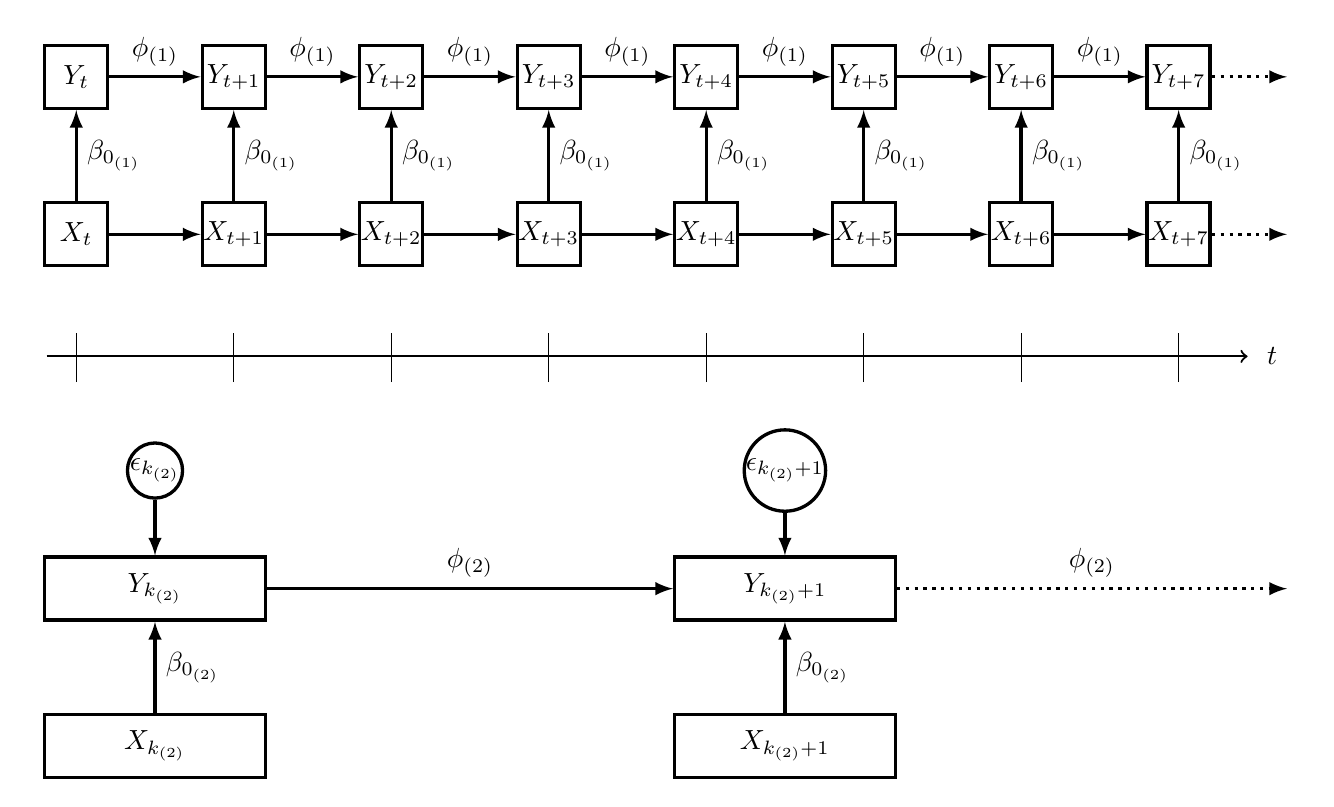
\begin{tikzpicture}[auto, scale = 0.5,
        time/.style={rectangle, inner sep=0pt, minimum size=8mm, align=center},
        manifest/.style={rectangle,draw,very thick,inner sep=0pt,minimum width=8mm,minimum height=8mm},
        paths/.style={->, very thick, -latex},
        resid/.style={circle, draw, very thick, inner sep=0pt, minimum size=7mm, align=center},
        double/.style={<->, very thick, -latex}
    ]
        % Nodes
        \node[manifest] (y0) at (0,0) {$Y_{t}$};
        \node[manifest, right of = y0, xshift = 1cm] (y1) {$Y_{t + 1}$};
        \node[manifest, right of = y1, xshift = 1cm] (y2) {$Y_{t + 2}$};
        \node[manifest, right of = y2, xshift = 1cm] (y3) {$Y_{t + 3}$};
        \node[manifest, right of = y3, xshift = 1cm] (y4) {$Y_{t + 4}$};
        \node[manifest, right of = y4, xshift = 1cm] (y5) {$Y_{t + 5}$};
        \node[manifest, right of = y5, xshift = 1cm] (y6) {$Y_{t + 6}$};
        \node[manifest, right of = y6, xshift = 1cm] (y7) {$Y_{t + 7}$};
        \node[right of = y7, xshift = 0.5cm] (y8) {};
                    
        \node[manifest, below of = y0, yshift = -1cm] (x0) {$X_{t}$};
        \node[manifest, below of = y1, yshift = -1cm] (x1) {$X_{t + 1}$};
        \node[manifest, below of = y2, yshift = -1cm] (x2) {$X_{t + 2}$};
        \node[manifest, below of = y3, yshift = -1cm] (x3) {$X_{t + 3}$};
        \node[manifest, below of = y4, yshift = -1cm] (x4) {$X_{t + 4}$};
        \node[manifest, below of = y5, yshift = -1cm] (x5) {$X_{t + 5}$};
        \node[manifest, below of = y6, yshift = -1cm] (x6) {$X_{t + 6}$};
        \node[manifest, below of = y7, yshift = -1cm] (x7) {$X_{t + 7}$};
        \node[below of = y8, yshift = -1cm] (x8) {};

        % Paths: Time-dependent effects
        \draw[paths] (x0) -- (y0) node[midway, right] {$\beta_{0_{(1)}}$};
        \draw[paths] (x1) -- (y1) node[midway, right] {$\beta_{0_{(1)}}$};
        \draw[paths] (x2) -- (y2) node[midway, right] {$\beta_{0_{(1)}}$};
        \draw[paths] (x3) -- (y3) node[midway, right] {$\beta_{0_{(1)}}$};
        \draw[paths] (x4) -- (y4) node[midway, right] {$\beta_{0_{(1)}}$};
        \draw[paths] (x5) -- (y5) node[midway, right] {$\beta_{0_{(1)}}$};
        \draw[paths] (x6) -- (y6) node[midway, right] {$\beta_{0_{(1)}}$};
        \draw[paths] (x7) -- (y7) node[midway, right] {$\beta_{0_{(1)}}$};

        % Paths: Autoregressive effects
        \draw[paths] (x0) -- (x1);
        \draw[paths] (x1) -- (x2);
        \draw[paths] (x2) -- (x3);
        \draw[paths] (x3) -- (x4);
        \draw[paths] (x4) -- (x5);
        \draw[paths] (x5) -- (x6);
        \draw[paths] (x6) -- (x7);
        \draw[paths, dotted] (x7) -- (x8);
                    
        \draw[paths] (y0) -- (y1) node[midway, above] {$\phi_{(1)}$};
        \draw[paths] (y1) -- (y2) node[midway, above] {$\phi_{(1)}$};
        \draw[paths] (y2) -- (y3) node[midway, above] {$\phi_{(1)}$};
        \draw[paths] (y3) -- (y4) node[midway, above] {$\phi_{(1)}$};
        \draw[paths] (y4) -- (y5) node[midway, above] {$\phi_{(1)}$};
        \draw[paths] (y5) -- (y6) node[midway, above] {$\phi_{(1)}$};
        \draw[paths] (y6) -- (y7) node[midway, above] {$\phi_{(1)}$};
        \draw[paths, dotted] (y7) -- (y8);
                    
        % Time line                
        \node (timeline-start) [below of = x0, yshift = -0.55cm, xshift = -.5cm] {};
        \node (timeline-end) [below of = x7, yshift = -0.55cm, xshift = 1cm] {};
             
        \draw[->, thick] (timeline-start) -- (timeline-end);
        \node at (timeline-end) [right] {$t$};  % Add letter t to the right of the timeline

        \node (t0) [below of = x0, yshift = -1cm] {};
        \node (t1) [below of = x1, yshift = -1cm] {};
        \node (t2) [below of = x2, yshift = -1cm] {}; 
        \node (t3) [below of = x3, yshift = -1cm] {}; 
        \node (t4) [below of = x4, yshift = -1cm] {}; 
        \node (t5) [below of = x5, yshift = -1cm] {}; 
        \node (t6) [below of = x6, yshift = -1cm] {}; 
        \node (t7) [below of = x7, yshift = -1cm] {}; 
             
        \foreach \tick in {t0, t1, t2, t3, t4, t5, t6, t7} {
            \draw (\tick) -- ++(0,1.5); 
        }
            
        % Nodes observed
        \node[resid, below of = t0, xshift = 1cm] (eyk0) {$\epsilon_{k_{(2)}}$};
        \node[resid, below of = t4, xshift = 1cm] (eyk1) {$\epsilon_{k_{(2)} + 1}$};
        
        \node[manifest, below of = eyk0, xshift = 0cm, yshift = -0.5cm, minimum width = 28mm] (yk0) {$Y_{k_{(2)}}$};
        \node[manifest, below of = eyk1, xshift = 0cm, yshift = -0.5cm, minimum width = 28mm] (yk1) {$Y_{k_{(2)} + 1}$};
        \node[right of = yk1, xshift = 5.5cm] (yk2) {};
                    
        \node[manifest, below of = yk0, yshift = -1cm, minimum width = 28mm] (xk0) {$X_{k_{(2)}}$};
        \node[manifest, below of = yk1, yshift = -1cm, minimum width = 28mm] (xk1) {$X_{k_{(2)} + 1}$};
        \node[right of = xk1, xshift = 5.5cm] (xk2) {};

        % Paths: Residuals
        \draw[paths] (eyk0) -- (yk0);
        \draw[paths] (eyk1) -- (yk1);

        % Paths: Time-dependent effects
        \draw[paths] (xk0) -- (yk0) node[midway, right] {$\beta_{0_{(2)}}$};
        \draw[paths] (xk1) -- (yk1) node[midway, right] {$\beta_{0_{(2)}}$};

        % Paths: Autoregressive effects
        \draw[paths] (yk0) -- (yk1) node[midway, above] {$\phi_{(2)}$};
        \draw[paths, dotted] (yk1) -- (yk2) node[midway, above] {$\phi_{(2)}$};
    \end{tikzpicture}
    \vspace{1cm}
    \caption{Above the timeline: A DAG of the data generating mechanism of Scenario 1. Below the timeline: A path diagram of the estimation model of Scenario 1 for the $m = 2$ aggregated data with sampling every two occasions. To avoid clutter, the (residual) variances and mean structure are not displayed in the path diagram.}
    \label{fig:scenario1}
\end{figure}

\subsubsection{3.1.3 Results} 
Bias and coverage probability (coverage) for the estimated $\beta_{0_{(1)}}$  across the experimental conditions are presented in Table~\ref{tab:scenario1-results}, in the columns under ``Scenario 1''. Figure~\ref{fig:scenario1-results-beta0} visualizes the sampling distribution of the estimate of $\beta_{0}$. The impact of time-aggregation on the estimated $\beta_{0_{(1)}}$ can be seen by comparing results across the different rows for a given column; the impact of systematic sampling can be evaluated by comparing results across the different columns for a given row. Numerical results and visualizations of sampling distributions for estimates of the autoregressive effect can be found in Appendix~\ref{app:simulation-scenario1}.

First we inspect results for the experimental condition where the temporal characteristics of the data and the data generating process align, that is $m = 1$ and sampling every first observation. Estimates for $\beta_{0}$ and $\phi$ using the model of Equation~\ref{eq:scenario1-estimation} show no bias and good coverage. This implies that the estimation model is sufficient to estimate the causal effect of interest and the autoregressive effect when the temporal characteristics of the data and the effect of interest are aligned. 

Second, we inspect the effect of time-aggregation, holding the sampling scheme constant. In the condition where data were sampled every first observation, time-aggregation introduces an upward bias for the estimated $\beta_{0}$, leading to estimates with an average of $0.925$ (Monte Carlo standard error, MC-SE = 0.003) and a coverage rate of the 95\% confidence interval of 0.018 for the case of time aggregation over $m = 10$ periods. A similar upward bias due to the impact of time-aggregation exists for other systematic (under)sampling schemes---that is, sampling every second, third, fifth, or tenth observation---as well. 

Third, when inspecting the effect of systematic (under)sampling for a given time-aggregation scheme, it can be seen that the systematic sampling itself also introduces an upward bias for the estimates of $\beta_{0}$. That is, for a given aggregation scheme (row), the average estimate of $\beta_{0}$ shows a positive bias when sampling only every second, third, fifth, or tenth observation. This can be explained by the intermitted exposure variables $X$ that remain unobserved as a result of the systematic (under)sampling, and that act as confounders for the effect $\beta_{0}$. Combined, the time-aggregation and systematic sampling result in an average estimate for $\beta_{0}$ of $0.936$ (MC-SE $= 0.003$) with a coverage rate of the 95\% confidence intervals of 0.018 for the case of sampling every 10th occasion and time-aggregation over $m = 10$ periods, whereas the true population value is $\beta_{0} = 0.5$. 

 \begin{table}[]
    \centering
    \footnotesize
    \begin{tabular}[t]{ccccccc}
        \toprule
            &       & \multicolumn{2}{c}{Scenario 1} & & \multicolumn{2}{c}{Scenario 2} \\
        \cmidrule(lr){3-4} \cmidrule(lr){6-7}
        $m$ & Every & Avg. (MC-SE) & Cover. (MC-SE) & & Avg. (MC-SE) & Cover. (MC-SE) \\
        \midrule
        1 & 1 & 0.501 (0.002) & 0.965 (0.006) & & 0.5 (0.003) & 0.944 (0.007)\\
        1 & 2 & 0.599 (0.003) & 0.792 (0.013) & & 0.233 (0.003) & 0.168 (0.012)\\
        1 & 3 & 0.62 (0.003) & 0.75 (0.014) & & 0.052 (0.003) & 0.003 (0.002)\\
        1 & 5 & 0.621 (0.003) & 0.745 (0.014) & & -0.061 (0.003) & <0.000 (<0.000)\\
        1 & 10 & 0.625 (0.003) & 0.741 (0.014) & & -0.078 (0.003) & <0.000 (<0.000)\\
        \addlinespace
        2 & 1 & 0.649 (0.003) & 0.584 (0.016) & & 0.275 (0.003) & 0.347 (0.015)\\
        2 & 2 & 0.716 (0.003) & 0.363 (0.015) & & -0.157 (0.003) & <0.000 (<0.000)\\
        2 & 3 & 0.715 (0.003) & 0.401 (0.015) & & -0.24 (0.003) & <0.000 (<0.000)\\
        2 & 5 & 0.716 (0.003) & 0.388 (0.015) & & -0.246 (0.003) & <0.000 (<0.000)\\
        2 & 10 & 0.717 (0.003) & 0.388 (0.015) & & -0.249 (0.003) & <0.000 (<0.000)\\
        \addlinespace
        3 & 1 & 0.746 (0.003) & 0.249 (0.014) & & 0.062 (0.003) & 0.007 (0.003)\\
        3 & 2 & 0.776 (0.003) & 0.212 (0.013) & & -0.292 (0.003) & <0.000 (<0.000)\\
        3 & 3 & 0.77 (0.003) & 0.227 (0.013) & & -0.311 (0.003) & <0.000 (<0.000)\\
        3 & 5 & 0.775 (0.003) & 0.202 (0.013) & & -0.309 (0.003) & <0.000 (<0.000)\\
        3 & 10 & 0.775 (0.003) & 0.214 (0.013) & & -0.301 (0.003) & <0.000 (<0.000)\\
        \addlinespace
        5 & 1 & 0.839 (0.003) & 0.085 (0.009) & & -0.166 (0.003) & <0.000 (<0.000)\\
        5 & 2 & 0.854 (0.003) & 0.07 (0.008) & & -0.321 (0.003) & <0.000 (<0.000)\\
        5 & 3 & 0.859 (0.003) & 0.058 (0.007) & & -0.323 (0.003) & <0.000 (<0.000)\\
        5 & 5 & 0.849 (0.003) & 0.065 (0.008) & & -0.323 (0.003) & <0.000 (<0.000)\\
        5 & 10 & 0.853 (0.003) & 0.063 (0.008) & & -0.324 (0.003) & <0.000 (<0.000)\\
        \addlinespace
        10 & 1 & 0.925 (0.003) & 0.018 (0.004) & & -0.234 (0.003) & <0.000 (<0.000)\\
        10 & 2 & 0.927 (0.003) & 0.011 (0.003) & & -0.275 (0.003) & <0.000 (<0.000)\\
        10 & 3 & 0.928 (0.003) & 0.013 (0.004) & & -0.273 (0.003) & <0.000 (<0.000)\\
        10 & 5 & 0.927 (0.003) & 0.023 (0.005) & & -0.271 (0.003) & <0.000 (<0.000)\\
        10 & 10 & 0.936 (0.003) & 0.018 (0.004) & & -0.271 (0.003) & <0.000 (<0.000)\\
        \bottomrule
    \end{tabular}
    \caption{Average estimate and 95\% confidence interval coverage rate (including Monte Carlo standard errors) for estimates $\beta_{0}$ across experimental conditions in Scenarios 1 and 2.}
    \label{tab:scenario1-results}
\end{table}

\begin{figure}
    \centering
    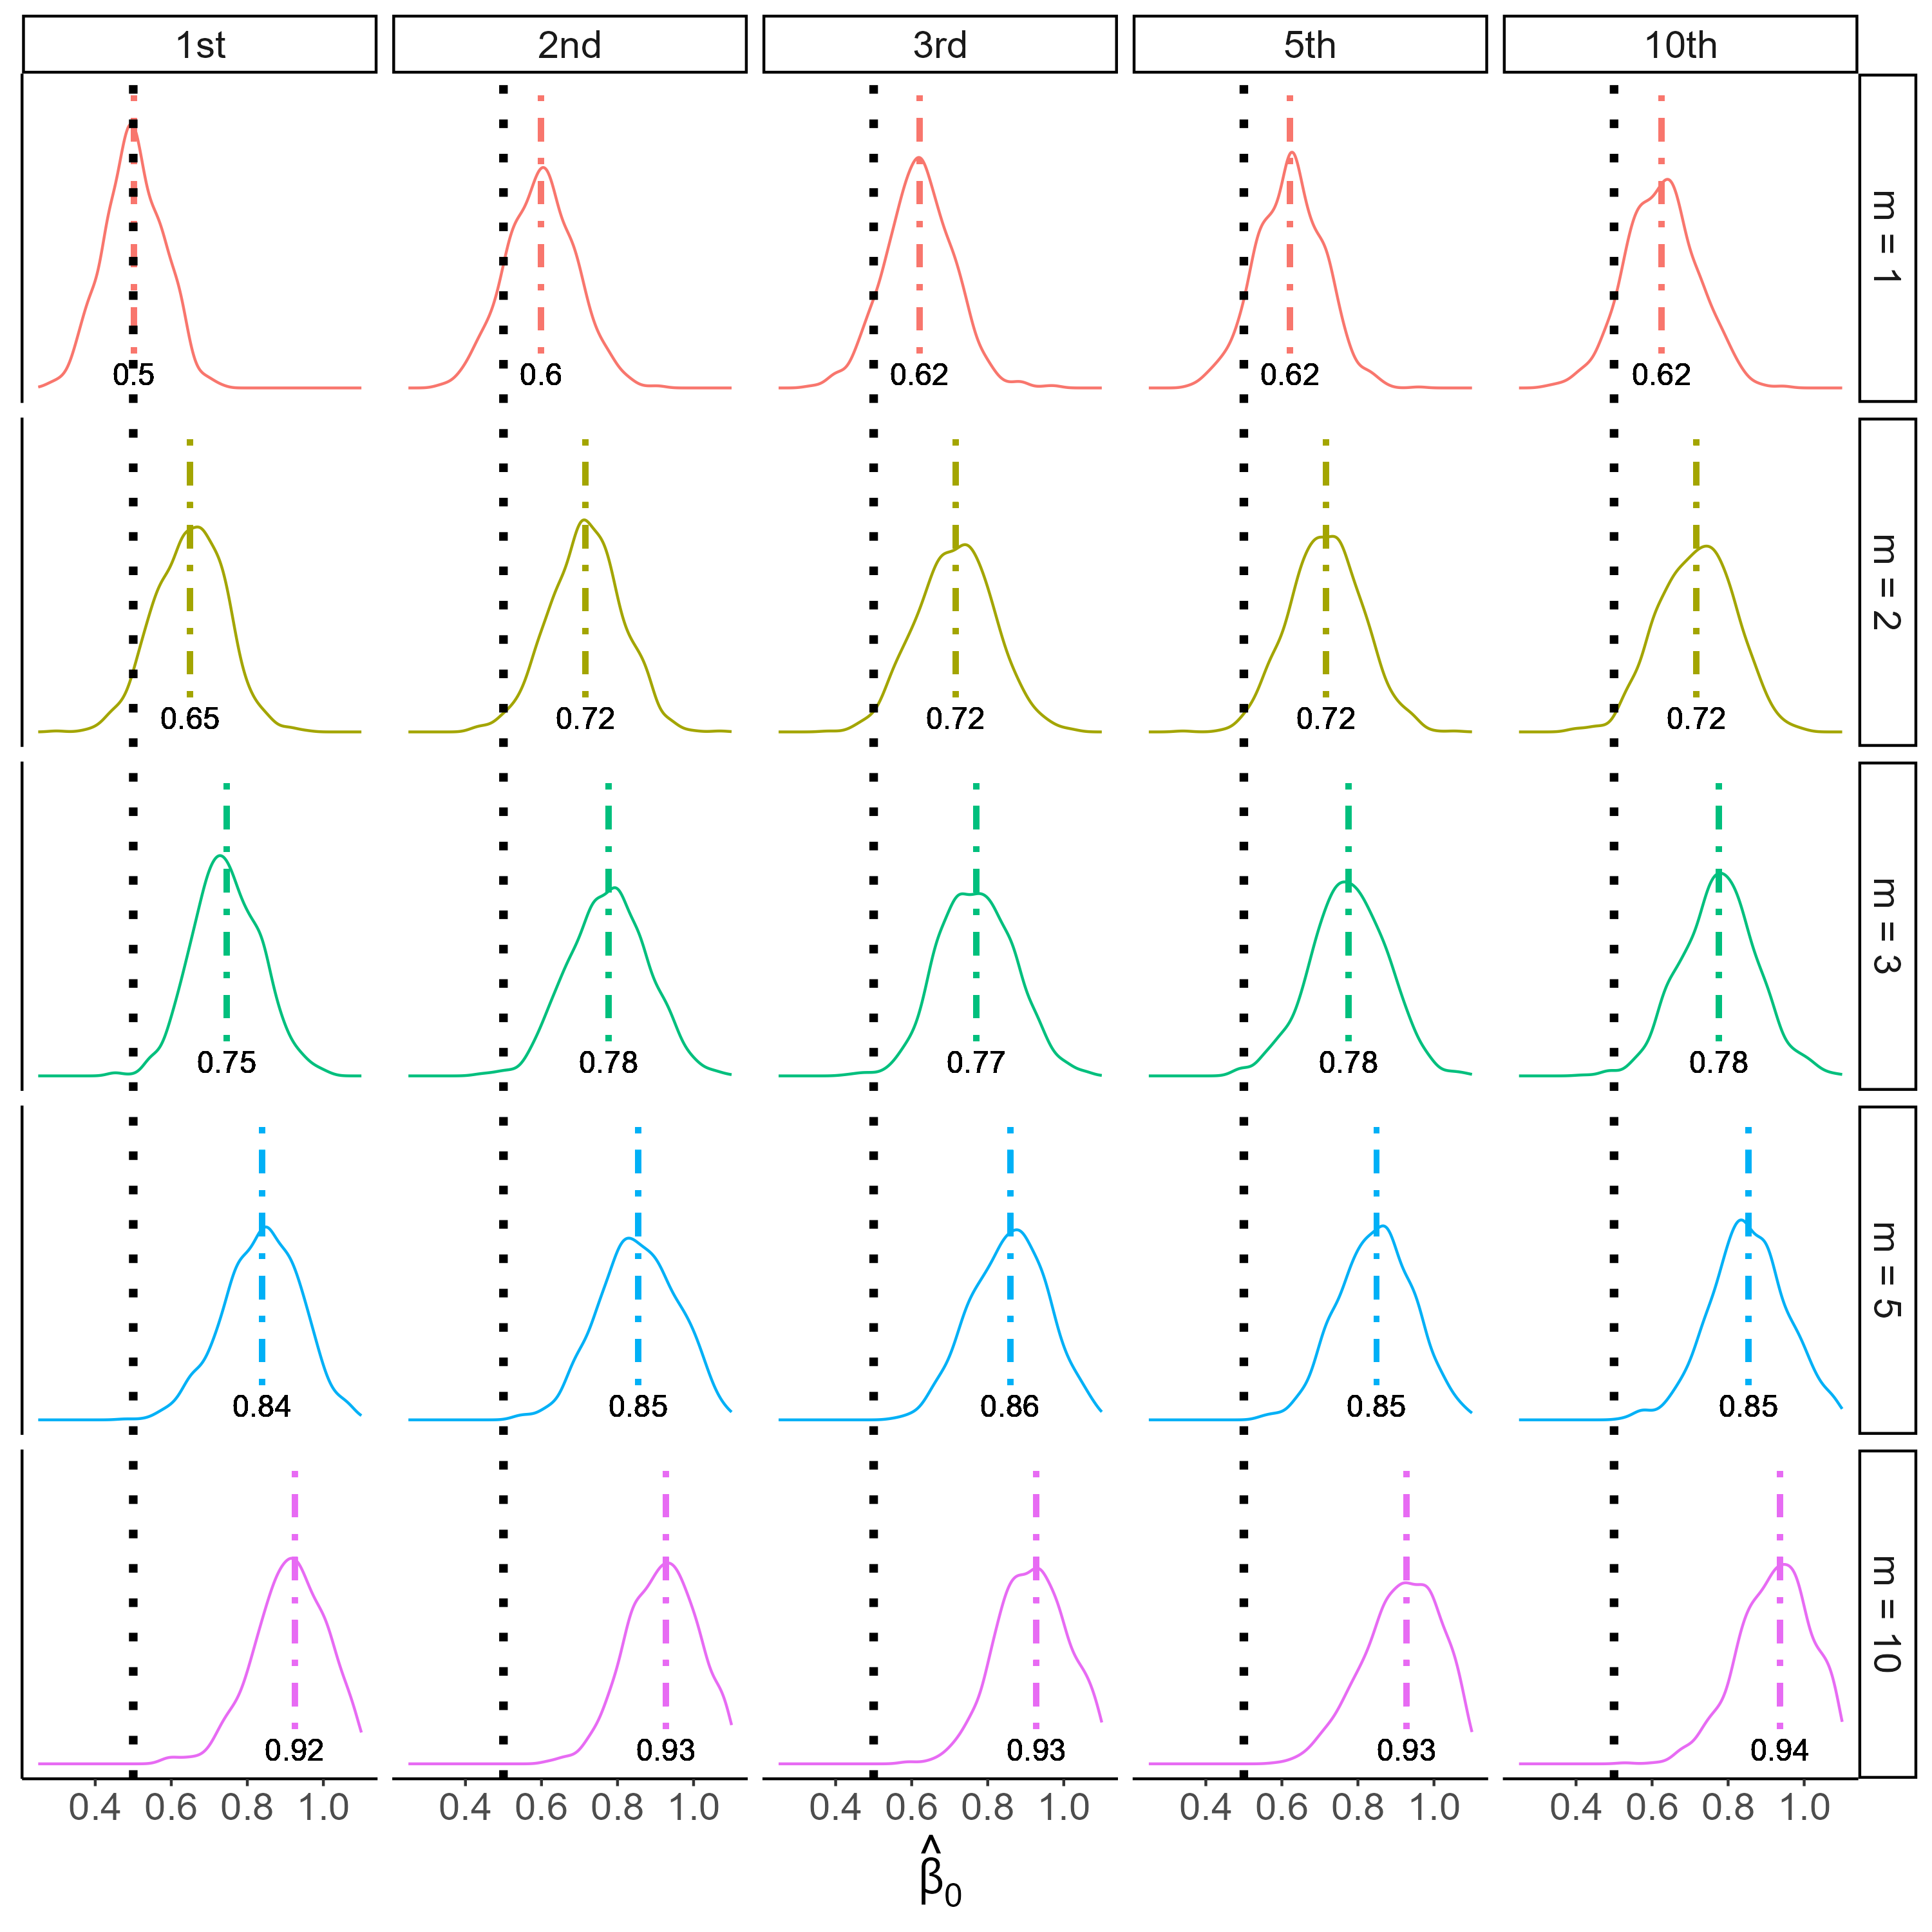
\includegraphics[width=1\linewidth]{figures/plot_scenario1_hats_beta0.png}
    \caption{Results Scenario 1: Sampling distribution of the estimated $\beta_{0}$ across experimental conditions. The columns ``1st'', ``2nd'', ``3rd'', ``5th'' and ``10th'' denote systematic sampling at every first, every second, every third, every fifth, and every tenth measurement occasion, respectively. Results are based on 1000 replications. The different rows represent time-aggregation across increasing numbers of time periods $m$. The black dotted line denotes the population value $\beta_{0} = 0.5$. The colored dot-stripe lines denote the average parameter estimate per experimental condition.}
    \label{fig:scenario1-results-beta0}
\end{figure}

\subsection{3.2 Scenario 2}
When the aim of a study is causal inference, researchers typically have to control for covariates to identify the causal effect of interest. Therefore, in Scenario 2, the data generating mechanism of Scenario 1 is extended with a time-varying covariate $L$. In the context of our empirical example, this could represent daily amount of alcohol or drug usage \parencite{feder_is_2020}. 

\subsubsection{3.2.1 Data Generation}
Suppose that $L_{t}$ is a continuous time-varying covariate that influences $X_{t}$ and $Y_{t}$ within a day, and itself has an autoregressive structure. The top of Figure~\ref{fig:scenario2} illustrates this data generating mechanism. Let $L_{t}$ be generated by
\begin{equation*} \label{eq:scenario2-DGM-L}
    L_{t} = \alpha L_{t - 1} + \epsilon_{L,t},
\end{equation*}
with $\alpha = 0.5$ and the residual $\epsilon_{L, t}$ normally distributed with variance set to $\sigma_{L}^{2} = 1$. To have the time-varying covariate $L_{t}$ influence the exposure $X_{t}$, we make the transition probabilities of the exposure dependent on the previous outcome $Y$ and current covariate $L$. Depending on the current state of the exposure $X_{t}$, the next exposure state $X_{t + 1}$ is given by the logistic regression models 
\begin{align*} 
    p(X_{t + 1} = 1 | X_{t} = 0) &= expit(\delta_{10, 0} + \delta_{10, 1} Y_{t} + \delta_{10, 2} L_{t + 1}), \\ 
    p(X_{t + 1} = 0 | X_{t} = 1) &= expit(\delta_{01, 0} + \delta_{01, 1} Y_{t} + \delta_{01, 2} L_{t + 1}),
\end{align*}
where $expit(\cdot) = \frac{1}{1 + exp(-(\cdot))}$. Parameter values for the transition from state 0 to state 1 were set to $\delta_{10, 0} = -2$, representing a high baseline probability of remaining in state 0, $\delta_{10, 1} = -0.5$, implying a negative effect of anxiety on social media use (i.e., increased anxiety decreases likelihood of subsequent social media use), and $\delta_{10, 2} = 1$, representing a positive effect of the covariate on likelihood of social media use. Parameter values for the transition from state 1 to state 0 were set to $\delta_{01, 0} = 0$, representing an even baseline probability of switching to ``no social media use'', and $\delta_{01, 1} = 1$ and $\delta_{01, 2} = 1$, implying that increased stress and covariate values increase the likelihood of switching to ``no social media use''. The outcome is generated following
\begin{equation} \label{eq:scenario2-DGM-Y}
    Y_{it} = \phi Y_{t - 1} + \beta_{0} X_{it} + \gamma_{0} L_{t} + \epsilon_{Y,t}
\end{equation}
with $\gamma_{0} = 0.8$. $\phi$, $\beta_{0}$, and $\sigma_{Y}^{2}$ were set to the same population values as in Scenario 1. 

To create $X_{k_{(m)}}$, $L_{k_{(m)}}$, and $Y_{k_{(m)}}$, we aggregate the generated data over $m = 1, 2, 3, 5, 10$ periods and systematically sampled every first, every second, and every third, every fifth, and every 10th time point. Again, the total number of time points $T$ was adjusted per experimental condition to ensure a thousand observations per condition. 

\begin{figure}
    \centering
    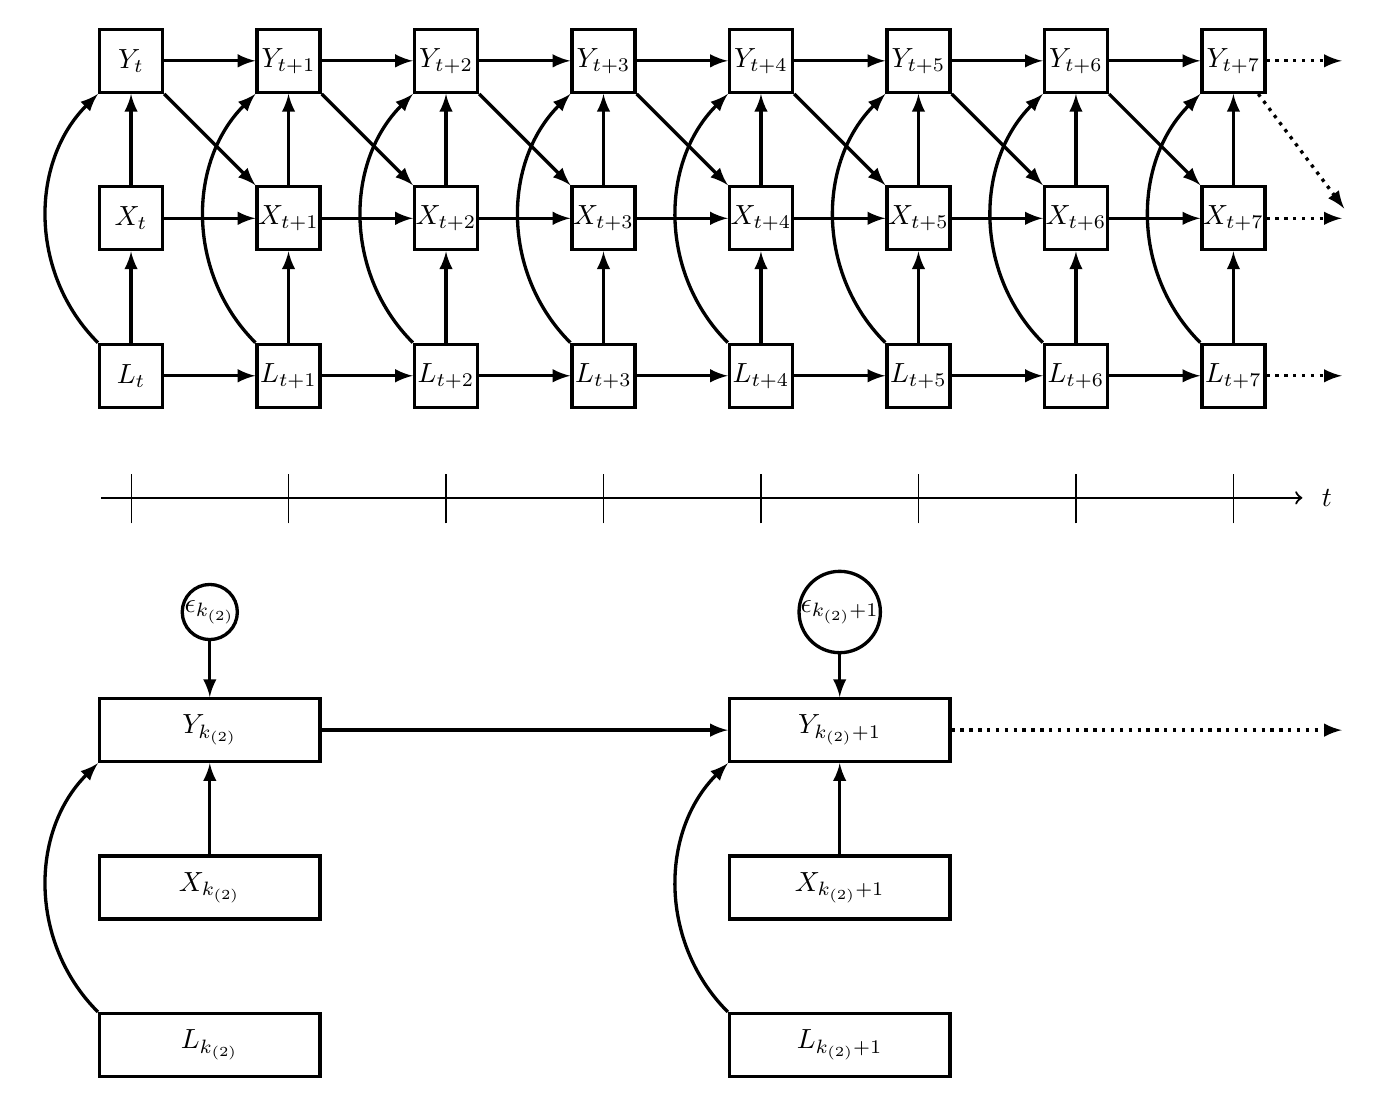
\begin{tikzpicture}[auto, scale = 0.5,
        time/.style={rectangle, inner sep=0pt, minimum size=8mm, align=center},
        manifest/.style={rectangle,draw,very thick,inner sep=0pt,minimum width=8mm,minimum height=8mm},
        paths/.style={->, very thick, -latex},
        resid/.style={circle, draw, very thick, inner sep=0pt, minimum size=7mm, align=center},
        double/.style={<->, very thick, -latex}
    ]
        % Nodes
        \node[manifest] (y0) at (0,0) {$Y_{t}$};
        \node[manifest, right of = y0, xshift = 1cm] (y1) {$Y_{t + 1}$};
        \node[manifest, right of = y1, xshift = 1cm] (y2) {$Y_{t + 2}$};
        \node[manifest, right of = y2, xshift = 1cm] (y3) {$Y_{t + 3}$};
        \node[manifest, right of = y3, xshift = 1cm] (y4) {$Y_{t + 4}$};
        \node[manifest, right of = y4, xshift = 1cm] (y5) {$Y_{t + 5}$};
        \node[manifest, right of = y5, xshift = 1cm] (y6) {$Y_{t + 6}$};
        \node[manifest, right of = y6, xshift = 1cm] (y7) {$Y_{t + 7}$};
        \node[right of = y7, xshift = 0.5cm] (y8) {};
                    
        \node[manifest, below of = y0, yshift = -1cm] (x0) {$X_{t}$};
        \node[manifest, below of = y1, yshift = -1cm] (x1) {$X_{t + 1}$};
        \node[manifest, below of = y2, yshift = -1cm] (x2) {$X_{t + 2}$};
        \node[manifest, below of = y3, yshift = -1cm] (x3) {$X_{t + 3}$};
        \node[manifest, below of = y4, yshift = -1cm] (x4) {$X_{t + 4}$};
        \node[manifest, below of = y5, yshift = -1cm] (x5) {$X_{t + 5}$};
        \node[manifest, below of = y6, yshift = -1cm] (x6) {$X_{t + 6}$};
        \node[manifest, below of = y7, yshift = -1cm] (x7) {$X_{t + 7}$};
        \node[below of = y8, yshift = -1cm] (x8) {};

        \node[manifest, below of = x0, yshift = -1cm] (l0) {$L_{t}$};
        \node[manifest, below of = x1, yshift = -1cm] (l1) {$L_{t + 1}$};
        \node[manifest, below of = x2, yshift = -1cm] (l2) {$L_{t + 2}$};
        \node[manifest, below of = x3, yshift = -1cm] (l3) {$L_{t + 3}$};
        \node[manifest, below of = x4, yshift = -1cm] (l4) {$L_{t + 4}$};
        \node[manifest, below of = x5, yshift = -1cm] (l5) {$L_{t + 5}$};
        \node[manifest, below of = x6, yshift = -1cm] (l6) {$L_{t + 6}$};
        \node[manifest, below of = x7, yshift = -1cm] (l7) {$L_{t + 7}$};
        \node[right of = l7, xshift = 0.5cm] (l8) {};

        % Paths: Time-dependent effects
        \draw[paths] (x0) -- (y0) node[midway, right] {};
        \draw[paths] (x1) -- (y1) node[midway, right] {};
        \draw[paths] (x2) -- (y2) node[midway, right] {};
        \draw[paths] (x3) -- (y3) node[midway, right] {};
        \draw[paths] (x4) -- (y4) node[midway, right] {};
        \draw[paths] (x5) -- (y5) node[midway, right] {};
        \draw[paths] (x6) -- (y6) node[midway, right] {};
        \draw[paths] (x7) -- (y7) node[midway, right] {};

        \draw[double](l0.north west) to [out=135, in=225] (y0.south west);
        \draw[double](l1.north west) to [out=135, in=225] (y1.south west);
        \draw[double](l2.north west) to [out=135, in=225] (y2.south west);
        \draw[double](l3.north west) to [out=135, in=225] (y3.south west);
        \draw[double](l4.north west) to [out=135, in=225] (y4.south west);
        \draw[double](l5.north west) to [out=135, in=225] (y5.south west);
        \draw[double](l6.north west) to [out=135, in=225] (y6.south west);
        \draw[double](l7.north west) to [out=135, in=225] (y7.south west);

        \draw[paths] (l0) -- (x0);
        \draw[paths] (l1) -- (x1);
        \draw[paths] (l2) -- (x2);
        \draw[paths] (l3) -- (x3);
        \draw[paths] (l4) -- (x4);
        \draw[paths] (l5) -- (x5);
        \draw[paths] (l6) -- (x6);
        \draw[paths] (l7) -- (x7);

        % Paths: Autoregressive effects
        \draw[paths] (x0) -- (x1);
        \draw[paths] (x1) -- (x2);
        \draw[paths] (x2) -- (x3);
        \draw[paths] (x3) -- (x4);
        \draw[paths] (x4) -- (x5);
        \draw[paths] (x5) -- (x6);
        \draw[paths] (x6) -- (x7);
        \draw[paths, dotted] (x7) -- (x8);
                    
        \draw[paths] (y0) -- (y1) node[midway, above] {};
        \draw[paths] (y1) -- (y2) node[midway, above] {};
        \draw[paths] (y2) -- (y3) node[midway, above] {};
        \draw[paths] (y3) -- (y4) node[midway, above] {};
        \draw[paths] (y4) -- (y5) node[midway, above] {};
        \draw[paths] (y5) -- (y6) node[midway, above] {};
        \draw[paths] (y6) -- (y7) node[midway, above] {};
        \draw[paths, dotted] (y7) -- (y8);

        \draw[paths] (l0) -- (l1);
        \draw[paths] (l1) -- (l2);
        \draw[paths] (l2) -- (l3);
        \draw[paths] (l3) -- (l4);
        \draw[paths] (l4) -- (l5);
        \draw[paths] (l5) -- (l6);
        \draw[paths] (l6) -- (l7);
        \draw[paths, dotted] (l7) -- (l8);

        % Lagged effects
        \draw[paths] (y0) -- (x1); 
        \draw[paths] (y1) -- (x2); 
        \draw[paths] (y2) -- (x3); 
        \draw[paths] (y3) -- (x4); 
        \draw[paths] (y4) -- (x5); 
        \draw[paths] (y5) -- (x6); 
        \draw[paths] (y6) -- (x7); 
        \draw[paths, dotted] (y7) -- (x8); 
                    
        % Time line                
        \node (timeline-start) [below of = l0, yshift = -0.55cm, xshift = -.5cm] {};
        \node (timeline-end) [below of = l7, yshift = -0.55cm, xshift = 1cm] {};
             
        \draw[->, thick] (timeline-start) -- (timeline-end);
        \node at (timeline-end) [right] {$t$};  % Add letter t to the right of the timeline

        \node (t0) [below of = l0, yshift = -1cm] {};
        \node (t1) [below of = l1, yshift = -1cm] {};
        \node (t2) [below of = l2, yshift = -1cm] {}; 
        \node (t3) [below of = l3, yshift = -1cm] {}; 
        \node (t4) [below of = l4, yshift = -1cm] {}; 
        \node (t5) [below of = l5, yshift = -1cm] {}; 
        \node (t6) [below of = l6, yshift = -1cm] {}; 
        \node (t7) [below of = l7, yshift = -1cm] {}; 
             
        \foreach \tick in {t0, t1, t2, t3, t4, t5, t6, t7} {
            \draw (\tick) -- ++(0,1.5); 
        }
            
        % Nodes observed
        \node[resid, below of = t0, xshift = 1cm] (eyk0) {$\epsilon_{k_{(2)}}$};
        \node[resid, below of = t4, xshift = 1cm] (eyk1) {$\epsilon_{k_{(2)} + 1}$};
        
        \node[manifest, below of = eyk0, xshift = 0cm, yshift = -0.5cm, minimum width = 28mm] (yk0) {$Y_{k_{(2)}}$};
        \node[manifest, below of = eyk1, xshift = 0cm, yshift = -0.5cm, minimum width = 28mm] (yk1) {$Y_{k_{(2)} + 1}$};
        \node[right of = yk1, xshift = 5.5cm] (yk2) {};
                    
        \node[manifest, below of = yk0, yshift = -1cm, minimum width = 28mm] (xk0) {$X_{k_{(2)}}$};
        \node[manifest, below of = yk1, yshift = -1cm, minimum width = 28mm] (xk1) {$X_{k_{(2)} + 1}$};
        \node[right of = xk1, xshift = 5.5cm] (xk2) {};

        \node[manifest, below of = xk0, yshift = -1cm, minimum width = 28mm] (lk0) {$L_{k_{(2)}}$};
        \node[manifest, below of = xk1, yshift = -1cm, minimum width = 28mm] (lk1) {$L_{k_{(2)} + 1}$};
        \node[right of = lk1, xshift = 5.5cm] (lk2) {};

         % Paths: Residuals
        \draw[paths] (eyk0) -- (yk0);
        \draw[paths] (eyk1) -- (yk1);

        % Paths: Time-dependent effects
        \draw[paths] (xk0) -- (yk0) node[midway, right] {};
        \draw[paths] (xk1) -- (yk1) node[midway, right] {};

        \draw[double](lk0.north west) to [out=135, in=225] (yk0.south west);
        \draw[double](lk1.north west) to [out=135, in=225] (yk1.south west);
                   
        \draw[paths] (yk0) -- (yk1) node[midway, above] {};
        \draw[paths, dotted] (yk1) -- (yk2) node[midway, above] {};
        
    \end{tikzpicture}
    \vspace{0.5cm}
    \caption{Above the timeline: A DAG of the data generating mechanism of Scenario 2. Below the timeline: A path diagram of the estimation model of Scenario 2, for the $m = 2$ aggregated data with sampling every two occasions. To avoid clutter, the (residual) variances and mean structure are not displayed in the path diagram.}
    \label{fig:scenario2}
\end{figure}

\subsubsection{3.2.2 Estimation}
The observed data are analyzed with a linear ARX(1) model, which is given by
\begin{equation} \label{eq:scenario2-estimation}
    Y_{k_{(m)}} = \phi_{(m)} Y_{k_{(m)} - 1} + \beta_{k_{(m)}} X_{k_{(m)}} + \gamma_{k_{(m)}} L_{k_{(m)}} + \epsilon_{Y,k_{(m)}}.
\end{equation}
The graph below the timeline in Figure~\ref{fig:scenario2} shows the path diagram belonging to this estimation model for the condition with $m = 2$ and systematically sampling every second frame. We assume the residuals $\epsilon_{Y,k_{(m)}}$ are normally distributed with a variance $\sigma^{2}_{Y}$. The model was fitted using DSEM in Mplus, version 8.11. Again, the interest lies in evaluating how informative the lag-0 parameter $\beta_{k_{m}}$ in the estimation model is about the lag-0 effect in the data generating mechanism. 

\subsubsection{3.2.3 Results}
The average estimate and 95\% coverage rate for estimates of $\beta_{0}$ across the experimental conditions are presented in Table~\ref{tab:scenario1-results}, in the columns under ``Scenario 2''. Figure~\ref{fig:scenario2-results-hats-beta0} displays the sampling distribution of the estimates of $\beta_{0_{(1)}}$ across experimental conditions in Scenario 2. Results for the parameters $\phi_{(m)}$ and $\gamma_{k_{(m)}}$ can be found Appendix~\ref{app:simulation-scenario2}.

Again, first inspecting the results for the experimental condition with $m = 1$ and sampling every first frame, we find no bias in the estimates of $\beta_{0_{(1)}}$ using the model in Equation~\ref{eq:scenario2-estimation}. This shows that under alignment of the temporal characteristics of the data and the data generating mechanism, adjustment for $X$ and $L$ at the same occasions and $Y$ at the previous occasion, is enough to identify the causal effect $\beta_{0_{(1)}}$. Second, focusing on the impact of time-aggregation and systematic (under)sampling, the results now show a downward bias for the estimated $\beta_{0_{(1)}}$. Given a sampling scheme in which every first frame is sampled, time-aggregation appears to introduce a downward bias for estimates of $\beta_{0_{(1)}}$, resulting in an average estimate of -0.234 (MC-SE $= 0.003$) and a coverage rate of $< 0.001$ for the case of aggregation over $m = 10$ periods. A similar downward bias exists for the systematic (under)sampling schemes of sampling every second, every third, every fifth, or every tenth frame.

Third, the systematic sampling similarly introduces a downwards bias for estimates $\beta_{0_{(1)}}$. That is, for any given time-aggregation scheme (i.e., a row in Figure~\ref{fig:scenario2-results-hats-beta0}), the bias becomes increasingly negative under systematically sampling every second, every third, etc. observation. In the experimental condition with time-aggregation across time time periods and systematically sampling every tenth frame, the average estimate of $\beta_{0}$ is even $-0.271$ (MC-SE $= 0.003$) with a coverage rate of zero. A reason for this large negative bias in this scenario might be that the effect of the time-varying confounder $L_{k}$ on the outcome $Y_{k}$ is severely overestimated, as can be seen in Appendix~\ref{app:simulation-scenario2}. The average estimate of $\gamma$ in the experimental condition with $m = 10$ and sampling every tenth frame is $1.270$, while the population value is $\gamma_{0} = 0.8$, implying an upward bias of $0.472$ (MC-SE $= 0.001$). It appears the large negative bias in $\beta_{0_{(1)}}$ might occur as a way to counter the large positive bias in estimates of $\gamma$. 

\begin{figure}
    \centering
    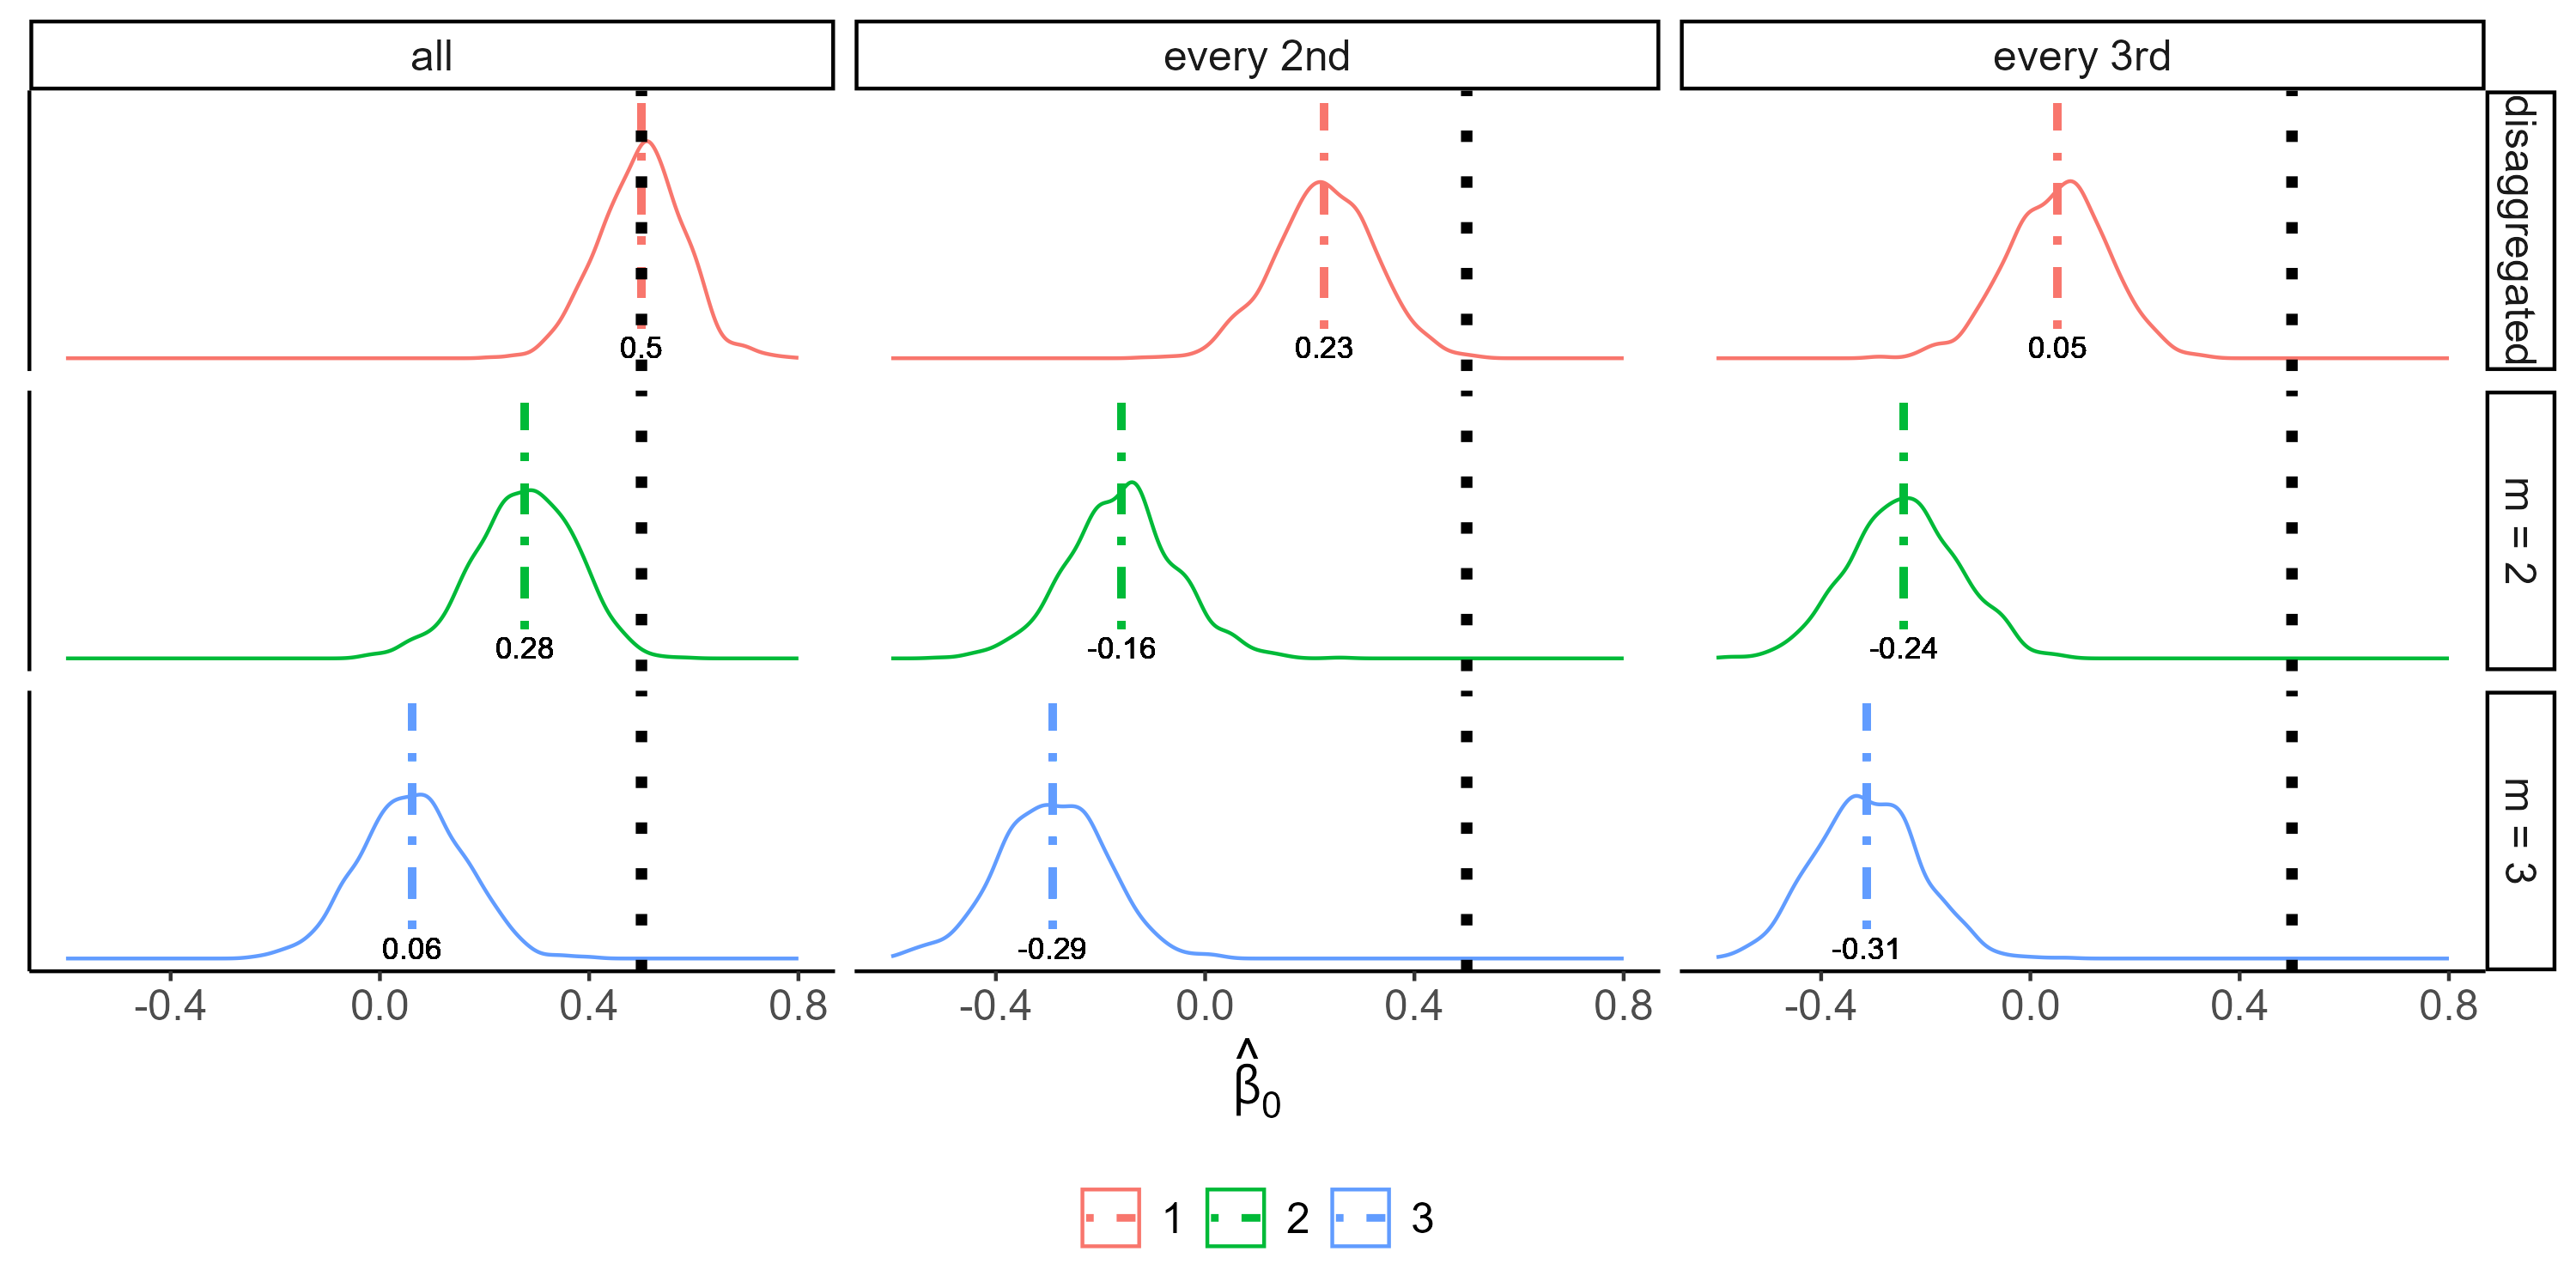
\includegraphics[width=1\linewidth]{figures/plot_scenario2_hats_beta0.png}
    \caption{Results Scenario 2: Sampling distribution of the estimated $\beta_{0}$ across experimental conditions.}
    \label{fig:scenario2-results-hats-beta0}
\end{figure}

\subsection{Scenario 3}
In Scenario 3, we extend the simulations of Scenario 2 to the context of panel data. That is, in Scenario 3 we use the same data generating mechanism as Scenario 2, but now generate data for multiple subjects, and changing the aggregation and systematic sampling scheme to be representative of panel data commonly found in psychology and related disciplines. 

\subsubsection{3.3.1 Data Generation}
Data are generated according to the data generating mechanism of Scenario 2, but now for multiple independent individuals. We inspect four experimental conditions, each involving a particular combination of time-aggregation and systematic sampling. Here, we take inspiration from different datasets concerning measures of self-esteem and depression that are included in \textcite{orth_testing_2021}, and specifically the research designs underlying these datasets as described in \textcite{hamaker_within-between_2023}. The first experimental condition reflects a research design with monthly measurement waves and with measurements of $X$, $L$, and $Y$ relating to the past week, that is, $m = 7$ and sampling only every fourth week. The second condition represents a case of annual measurements, and measurements of $X$, $L$, and $Y$ referring to ``the past month''. That is, we take $m = 30$ and sample every twelfth month. The third condition concerns a design with annual measurements, the measurements of which refer to ``the past year'', such that $m = 365$ and sampling every year. The fourth condition involves a design with biannual measurements and measurements referring to the past week, that is $m = 7$ and sampling every 102nd frame. In this design, less than 1\% of the process in $X$, $L$, and $Y$ is observed \parencite{hamaker_within-between_2023}. Finally, we also include an experimental condition with $m = 1$ and sampling every first frame. This is to verify that under alignment of the temporal dynamics of the data generating mechanism and the data, the effect $\beta_{0_{(1)}}$ is identified by the estimation method described in the next section. 

For all experimental conditions, we choose $T$ such that after time aggregation and systematic sampling, five repeated measures are available. The sample size was set to 500. Figure~\ref{fig:scenario3-data} illustrates the data for a single individual for the experimental condition with monthly measurements, and measurements referring to the past week. 

\begin{figure}
    \centering
    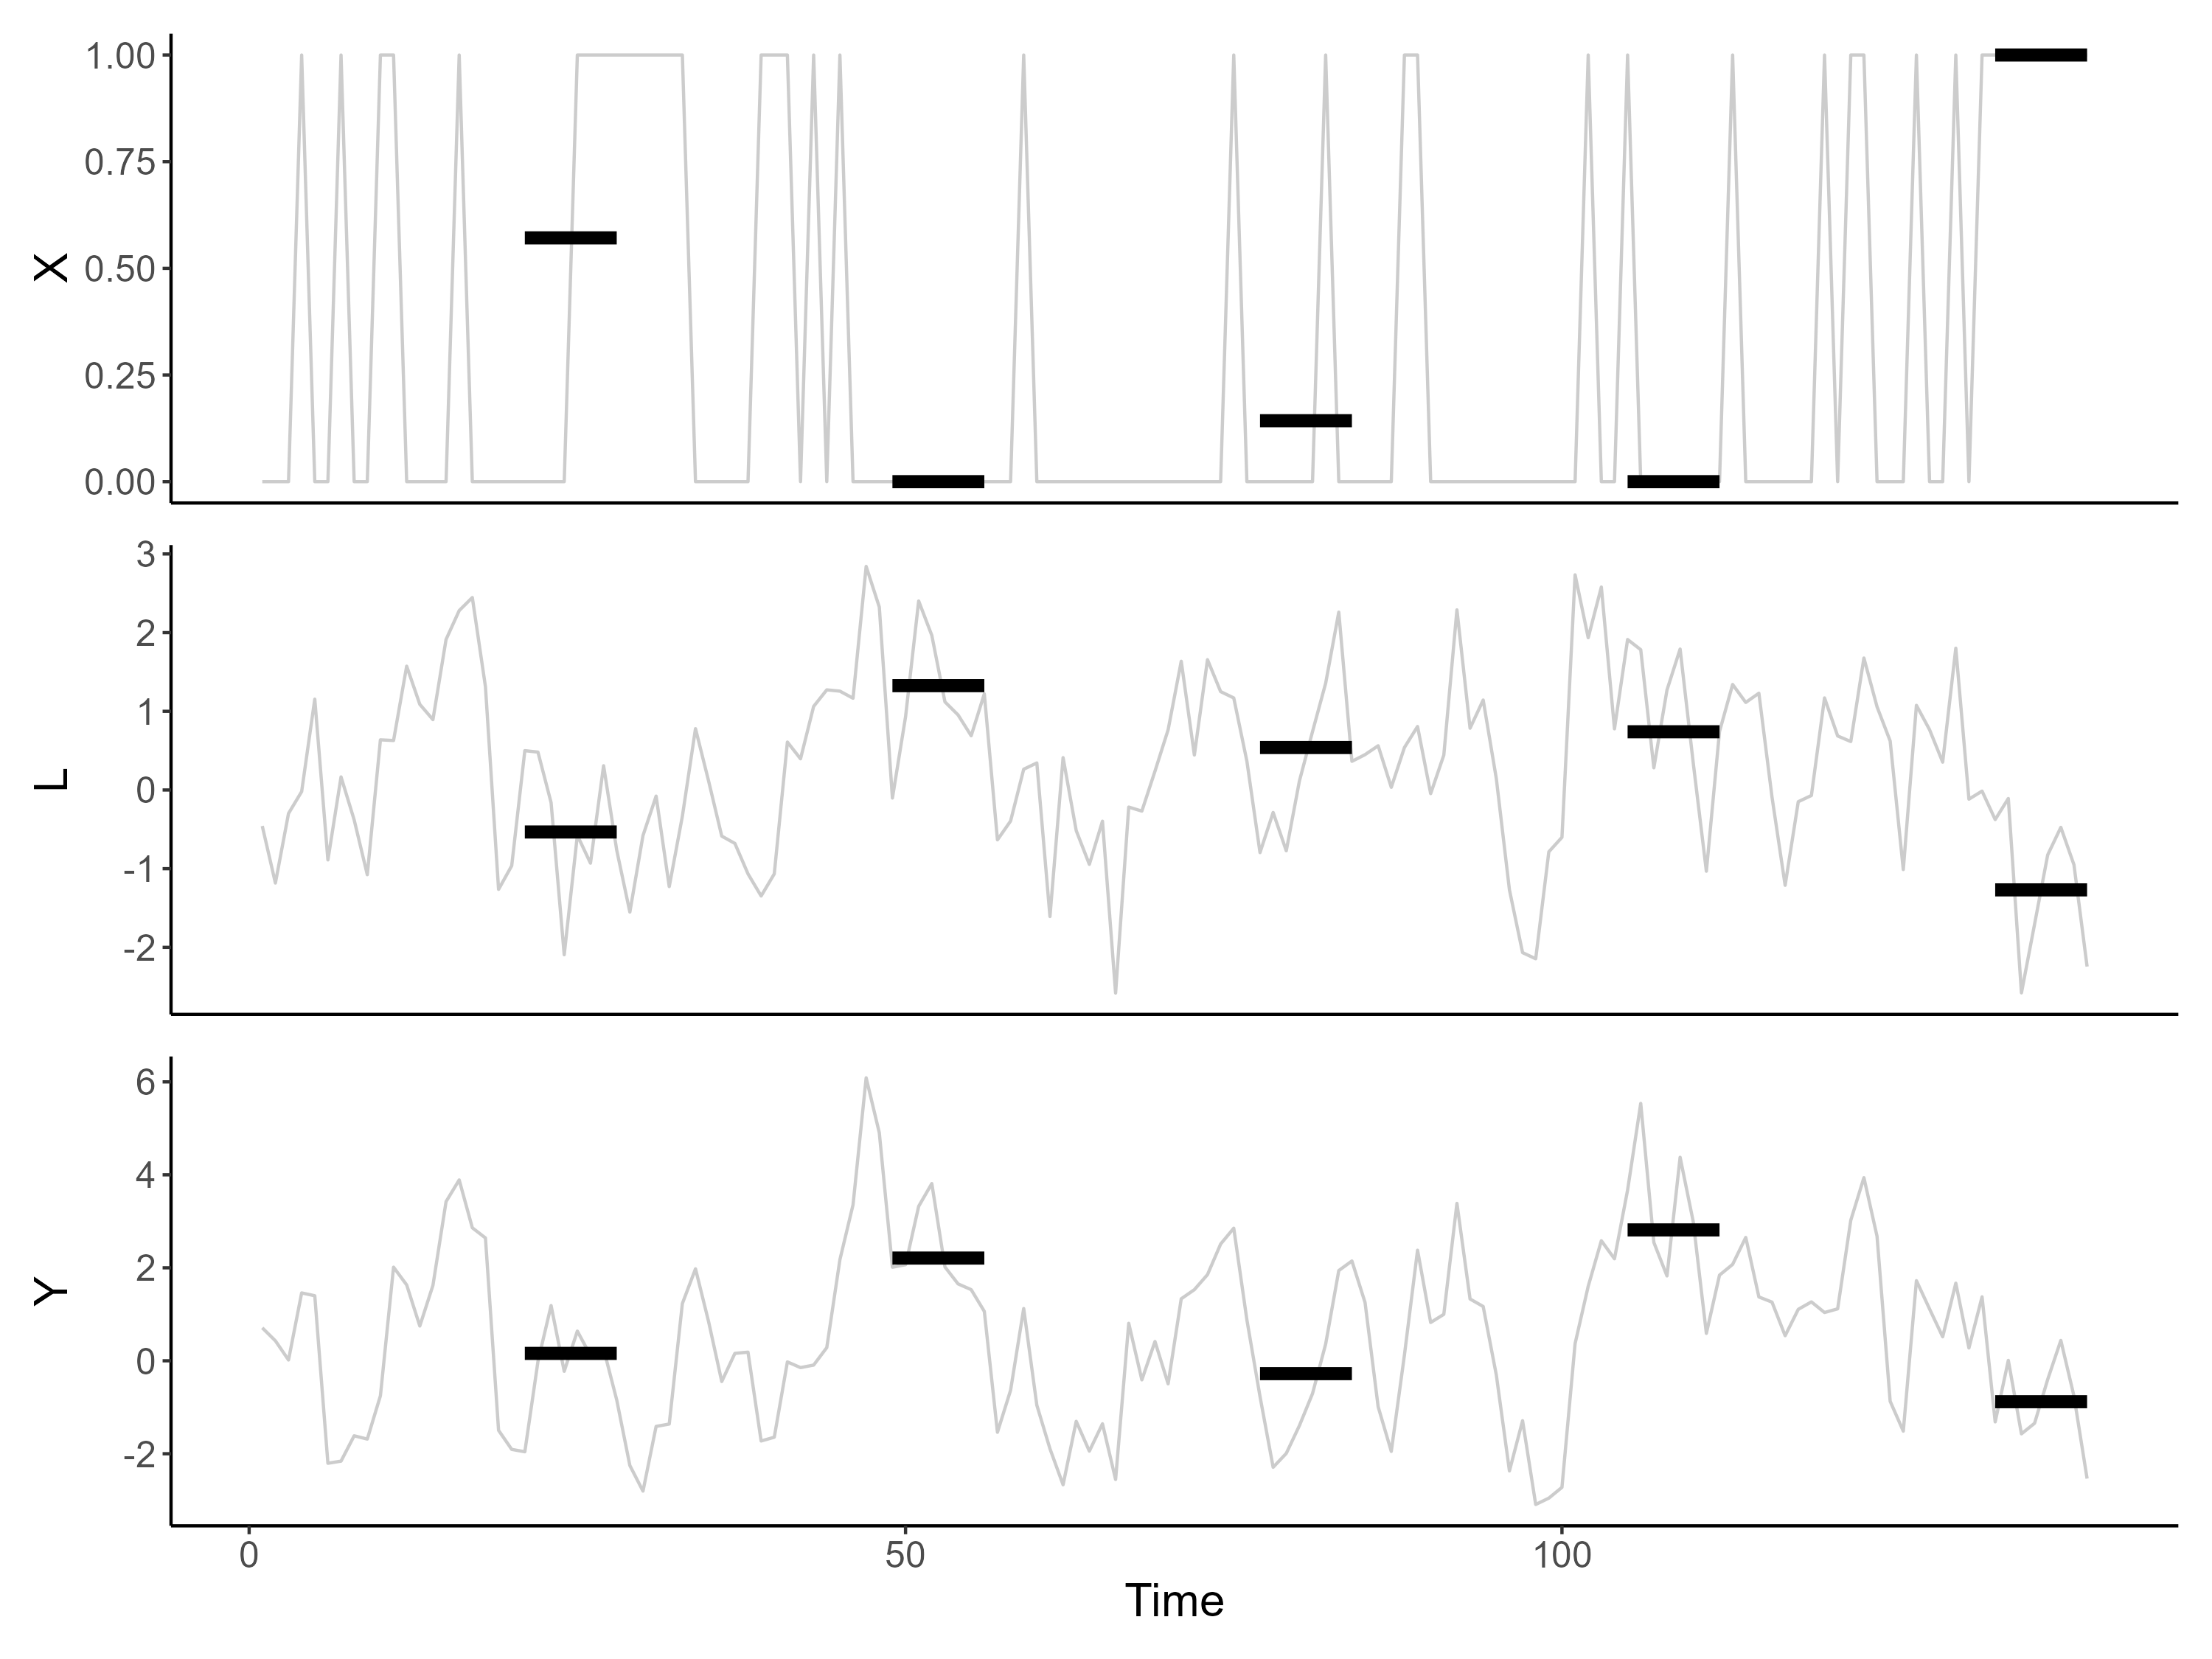
\includegraphics[width=0.9\linewidth]{figures/plot_scenario3_m7_every4.png}
    \caption{The disaggregated (gray lines) and observed aggregated data (bold black lines) for the time-varying exposure $X$, time-varying covariate $L$, and outcome $Y$ in Scenario 3, for the case of monthly measurements with time-aggregation per week.}
    \label{fig:scenario3-data}
\end{figure}

\subsubsection{3.3.2 Estimation}
Panel data with many individuals but few measurement occasions like in Scenario 3, necessitate a different modeling strategy compared to Scenarios 1 and 2. Within psychology, a popular approach is to analyse the data in wide-format using cross-lagged panel models within the structural equation modeling (SEM) framework \parencite{zyphur_data_2020, zyphur_data_2020-1, usami_unified_2019}. As we are only interested in the effect of social media use on stress, we made use of unidirectional versions of these models. Specifically, we specified a wide-format ARX(1) model in the SEM framework in which $Y_{k_{(m)}}$ is predicted by $X_{k_{(m)}}$ and $L_{k_{(m)}}$, which can be represented equivalently to Equation~\ref{eq:scenario2-estimation}. The lag-0 effects from $L_{k_{(m)}}$ and $X_{k_{(m)}}$ were constrained to be time-invariant. The time-varying exposure $X_{k_{(m)}}$ and covariate $L_{k_{(m)}}$ were allowed to freely covary with each other over time. The wide-format ARX(1) is estimated in the SEM framework using the R package lavaan \parencite[version 0.6-18;][]{rosseel_lavaan_2012}.  

\subsubsection{3.3.3 Results}
The average estimate and 95\% coverage rate for the estimates of $\beta_{0{(1)}}$ are presented in Table~\ref{tab:scenario3-results}. Results for the parameters $\phi_{(m)}$ and $\gamma_{(m)}$ can be found Appendix~\ref{app:simulation-scenario3}. First, looking at the results for $\beta_{0{(1)}}$ in the experimental condition with $m = 1$ and sampling every first frame, we find that the wide-format ARX(1) model on average estimates an effect of $0.498$, implying no bias in the estimates of $\beta_{0{(1)}}$ using this modeling strategy. The 95\% confidence interval (CI) coverage rate is estimated at $0.926$ with a Monte Carlo standard error (MC-SE) of $0.008$. This is a little below the expected coverage rage of $0.95$, but could be due to sampling fluctuations in the simulations. 

Results for the other experimental conditions in this scenario mirror the results of Scenario 2. For monthly measurement of variables that have been aggregated over weeks ($m = 7$), the average estimate is $-0.301$ (MC-SE $= 0.002$) with a coverage rate of zero, which is far off from the $X$ to $Y$ effect that generated the data. This implies that in practice, under this research design, researchers might conclude that there exists a negative effect of social media use on stress (i.e., social media reduces one's stress levels) whereas, in fact, the causal mechanism that generated the data included a positive effect. When week-aggregates ($m = 7$) are collected biannually instead (i.e., a measurement every 102nd week)---that is, less than 1\% off the causal process has been observed----the bias and 95\% coverage rate are relatively similar. For the condition with aggregation over the past month ($m = 30$) and yearly measurements, the average estimate is $-0.208$ (MC-SE $= 0.002$) with a coverage rate of zero again. Finally, a research design with measurements that aggregate over the past year $m = 365$ and takes measurements annually, the estimates are similarly off from $\beta_{0_{(1)}}$ in the data generating mechanism: The average estimate is $-0.177$ (MC-SE $= 0.002$) with a 95\% coverage rate of $< 0.000$. 

 \begin{table}[]
    \centering
    \footnotesize
    \begin{tabular}[t]{cccc}
        \toprule
        $m$ & Every & Avg. (MC-SE) & Cover. (MC-SE)\\
        \midrule
        1 & 1 & 0.498 (0.002) & 0.926 (0.008)\\
        7 & 4 & -0.301 (0.002) & <0.000 (<0.000)\\
        7 & 102 & -0.299 (0.002) & <0.000 (<0.000)\\
        30 & 12 & -0.208 (0.002) & <0.000 (<0.000)\\
        365 & 1 & -0.177 (0.002) & <0.000 (<0.000)\\
        \bottomrule
    \end{tabular}
    \caption{Average estimate and 95\% confidence interval coverage rate (including Monte Carlo standard errors) for estimates $\beta_{0}$ across experimental conditions in Scenario 3.}
    \label{tab:scenario3-results}
\end{table}

\section{4. Discussion}
Time-aggregation of measurements and low process coverage due to systematic (under)sampling over time are two very common temporal features of panel data. A specific time-aggregation or systematic sampling scheme can be selected in the design of a longitudinal study for a diverse set of methodological and practical reasons \parencites{dollard_timing_2014, janssens_qualitative_2018}. For example, aggregation is sometimes used as a method for dealing with measurement error \parencite{rushton_behavioral_1983} and increasing the interval between repeated measures decreases participant burden while still enabling researchers to measure participants over extended periods of time. However, more generally, substantive literature and theories in the social sciences are notoriously uninformative about the time scale at which to measure a process of interest \parencite{collins_analysis_2006, dormann_optimal_2015}. For this reason, \textcite[p. 533]{mitchell_building_2001} have stated that decisions about the time scale of a study design are often ``(...) left to intuition, chance, convenience, or tradition'', and \textcite[p. S85]{collins_effect_2002} express concern about the lack of awareness about the impact of uninformed temporal design choices on the results of a study: \begin{quote} ``Scientific, theoretical, or conceptual, as opposed to logistical, reasons for the choice of temporal design are rarely mentioned, and equally rare is any discussion of how this choice might have affected the statistical and substantive conclusions drawn from the study.'' \end{quote} Similarly, \textcite{voelkle_role_2018} discuss how researchers can arrive at different conclusions depending on different data collection designs, concluding that without due consideration of time, studying psychological mechanisms is next to impossible. 

The aim of this paper was therefore to demonstrate the impact of time-aggregation and systematic sampling on a researchers ability to study the causal mechanism that underlies a particular relationship of interest, specifically when the causal mechanism takes places at a finer time scale than the observed data. While the topic of time-aggregation has received some attention in the econometric literature for dynamic models, it has been severely understudied in the social sciences. For relatively simple autoregressive processes such as the AR(1) and ARX(1) with one time-dependent covariate, there exists some analytical work on time-aggregation and systematic sampling. For example, it can be analytically derived how the autoregressive effect of a stationary disaggregated AR(1) process, and the autoregressive effect and the effect of the time-dependent predictor of a disaggregated ARX(1) process, are related to the parameters that can be obtained from aggregated data \parencite[cf.][]{amemiya_effect_1972, brewer_consequences_1973}. Furthermore, in the time-series literature it is well-described how parameters of dynamic models change when the time-interval between repeated measures changes \parencite[e.g., due to systematic (under)sampling;][]{chatfield_analysis_2003}. However, deriving analytically their combined impact for slightly more complex models is challenging \parencite{amemiya_effect_1972, petkovic_aggregation_2009}. We therefore presented simulation results for three different scenarios, which include (a) a bivariate process with a time-varying exposure and outcome for $N = 1$; (b) a process with time-varying exposure, outcome, and covariate for $N = 1$; and (c) a process with a time-varying exposure, outcome, and covariate for panel designs that include multiple individuals, but fewer time points per individual. Each scenario contained experimental conditions with varying levels of time-aggregation and systematic (under)sampling. For each experimental condition, we evaluated how well parameter estimates based on observed data approximate the parameters that govern the data generating mechanism, focussing specifically on the causal effect of $X_{t}$ on $Y_{t}$, $\beta_{0_{(1)}}$. 

We have shown that a mismatch between the temporal characteristics of a causal process and the time-scale of the observed data can lead to over- and underestimation of estimates of $\beta_{0}$. The direction and size of the bias, however, is naturally very much dependent on the underlying causal process. For Scenario 1, we observed an upwards bias as a result of both systematic (under)sampling and time-aggregation of the variables. Combined, this resulted in conditions in which parameters estimates of the lag-0 effect of $X_{k_{(m)}}$ on $Y_{k_{(m)}}$ are not reflective anymore of the parameters that govern the data generating mechanism, and the 95\% CI coverage rate approached zero as the aggregation period and systematic (under)sampling increased. In this scenario and for our empirical example, it would imply that applied researchers working with aggregated and undersampled data might conclude that there are strong lag-0 effects of social media use on stress levels whereas, in fact, these are (much) smaller in the data generating mechanism. In contrast, for Scenarios and 2 and 3, we found a strong negative bias in the estimates of $\beta_{0_{(m)}}$, resulting in average estimates that were negative and had a 95\% CI coverage rate of zero. In these situations and in the context of the empirical example, applied researchers might conclude that there exists a negative instantaneous effect of social media use on stress levels based on aggregated and undersampled data. A naive interpretation of these results (i.e., not considering or unawareness of how the temporal design of the study affected statistical results) can then lead to wrong, and potentially harmful advice.  

\subsection{4.1 Implications}
In line with many previous methodological publications on this topic, this paper demonstrates the fundamental importance of making time scales a central aspect of substantive theories \parencite[cf.][]{hamaker_within-between_2023, mitchell_building_2001, dormann_optimal_2015, collins_effect_2002, driver_inference_2025}. While this point has been made predominantly when the interest was in identifying lag-1 cross-lagged effects in panel data or mediation analysis using SEM, this paper shows that it is at least equally important when the interest lies in lag-0 causal effects of a data generating mechanism. Or, stated a bit more provocatively, ``the effect of social media use on stress'' or ``the causal mechanism underlying the relationship between social media use and stress'' without linking the effect and mechanism to a time scale, do not exist. Without the specificity of the temporal characteristics of a causal process, it is also not possible to make an informed decision about how to optimally design an new panel study, nor is it possible to evaluate if an existing dataset contains the information needed to answer a research question \parencite{voelkle_role_2018}. For this reason, \textcite{collins_analysis_2006} argues that peer-review journals should request substantive researchers to provide a justification grounded in theoretical arguments for the time scale that was used in a study, and suggests that this is a necessary step for gaining insight into why particular findings in the literature fail to replicate. We agree with this argument. 

When theory offers little guidance on the temporal features of causal processes, a useful strategy might be to focus on the causal effects of ``policy interventions'' rather than on studying a ``causal mechanism''. That is, have the temporal features of a study design reflect the temporal features of the interventions (i.e., policy) that one hopes to inform with their causal research. For example, in the context of the empirical illustration, the ultimate goal of the research might be to inform an intervention where adults are blocked from using social media for a week, with the hope of reducing their stress levels at the end of that week (or throughout the entire week), compared to adults using social media at least once a day in a week. This is a different kind of causal research question, that focuses on contrasting outcomes that follow two different hypothesized interventions (akin to comparing outcomes from two different treatment arms in a randomized controlled trial), rather than the parameters in presumed underlying causal mechanism. Relating a research question to hypothesized practical interventions brings about concrete questions that researchers can answer to determine a useful research design: How long do I want my hypothesized interventions to be (e.g., a day, a week, a month)? In practice, how variable is social media use within the time frame of my hypothesized intervention (e.g., does social media use vary within a week)? when, after initiation of the hypothesized intervention, would I expect to see the effect if interest? How long do I want this effect to last? These questions are not intended to guide researchers to the ``true time scale'' of the causal process; rather, they help researchers to \textit{make decisions}, and target their research question to addressing the effects of practical interventions. This approach to asking causal questions is truly different from how many researchers in the field of psychology and related disciplines have been taught to think about causal inference; that is, causal inference as relating to differences in an outcome under two policy-interventions, rather than causal inferences as attempts to approximate values of parameters. Future research is needed to refine this approach, and explore its implications for different types of hypothesized interventions in a psychological context. 

\subsection{4.2 Limitations}
In this paper, we employ discrete-time models to estimate parameters of a ``true'' underlying day-to-day process based on aggregated and systematically (under)sampled data. In such settings, the observed bias might be (partly) remedied with smarter research design or analyses. One example, which we did not investigate in this manuscript, is the use of continuous-time modeling in combination with panel data that have been collected at varying time-intervals. \textcite{dormann_optimal_2015} already recommend to use varying time lags between repeated measures in the design of panel studies. They do so for a different reason, namely for computing the time lag at which the cross-lagged effect of $X$ to subsequent $Y$ is the biggest. However, this might also be a recommendable step considering the issue of unmeasured intermitted variables as a result of systematic (under)sampling and which confound the lag-0 effect $\beta_{0_{(1)}}$. In a research design with varying time lags, researchers can attempt to capture such intermitted variables in their sample. The continuous-time framework might then allow researchers to take the varying time lags into account and adjust for the confounding effect of intermitted time-varying confounders. However, the continuous-time framework is not commonly used in the context of confounder adjustment, and future research is needed to evaluate how well such an approach might work. 

A further limitation is that the simulation results in this paper are confined to the study of lag-0 effects. While this is a valid effect to study, interest in empirical research in the psychological and behavioral literature is typically on the lag-1 parameters in statistical models. The impact of time-aggregation and systematic (under)sampling is likely to be different for these kinds of effects. 

\subsection{4.3 Conclusion}
The alignment of the research question and data in a temporal sense is key in the study of causal mechanisms underlying psychological processes. Misalignment, due to time-aggregation of the variables and systematic (under)sampling can severely obscure a researcher's ability to identify and estimate parameters governing the causal mechanism, even resulting in estimates of the wrong sign, implying that wrong (and potentially harmful) conclusions can be draw. If theory offers little guidance on the temporal features of the causal mechanism, a useful strategy might be to ask a different causal question, guided by an interest in studying the effect of policy-interventions.

\printbibliography

\appendix

\section{Simulation Study: Additional Results} \label{app:simulation}


\subsection{Scenario 1} \label{app:simulation-scenario1}
Numerical results for the estimated autoregressive effect across the experimental conditions in Scenario 1 are presented in Table~\ref{tab:scenario1-results}. The column $\phi^{d}$ denotes what the expected autoregressive effect is when sampling every $d$th measurement occasion (i.e., the lag-$d$ effect). The coverage results for the estimates are computed based on $\phi^{d}$.

 \begin{table}[]
    \centering
    \footnotesize
    \begin{tabular}[t]{ccccc}
        \toprule
        $m$ & Every & $phi^{d}$ & Avg. (MC-SE) & Cover. (MC-SE)\\
        \midrule
        1 & 1 & 0.500 & 0.497 (0.001) & 0.948 (0.007)\\
        1 & 2 & 0.250 & 0.253 (0.001) & 0.952 (0.007)\\
        1 & 3 & 0.125 & 0.128 (0.001) & 0.957 (0.006)\\
        1 & 5 & 0.062 & 0.03 (0.001) & 0.813 (0.012)\\
        1 & 10 & 0.031 & -0.002 (0.001) & 0.812 (0.012)\\
        \addlinespace
        2 & 1 & 0.500 & 0.371 (0.001) & 0.001 (0.001)\\
        2 & 2 & 0.250 & 0.097 (0.001) & 0 (0)\\
        2 & 3 & 0.125 & 0.021 (0.001) & 0.077 (0.008)\\
        2 & 5 & 0.062 & 0 (0.001) & 0.456 (0.016)\\
        2 & 10 & 0.031 & -0.002 (0.001) & 0.796 (0.013)\\
        \addlinespace
        3 & 1 & 0.500 & 0.275 (0.001) & 0 (0)\\
        3 & 2 & 0.250 & 0.034 (0.001) & 0 (0)\\
        3 & 3 & 0.125 & 0.003 (0.001) & 0.022 (0.005)\\
        3 & 5 & 0.062 & -0.001 (0.001) & 0.451 (0.016)\\
        3 & 10 & 0.031 & -0.003 (0.001) & 0.806 (0.013)\\
        \addlinespace
        5 & 1 & 0.500 & 0.166 (0.001) & 0 (0)\\
        5 & 2 & 0.250 & 0.003 (0.001) & 0 (0)\\
        5 & 3 & 0.125 & -0.003 (0.001) & 0.017 (0.004)\\
        5 & 5 & 0.062 & -0.003 (0.001) & 0.418 (0.016)\\
        5 & 10 & 0.031 & -0.002 (0.001) & 0.801 (0.013)\\
        \addlinespace
        10 & 1 & 0.500 & 0.074 (0.001) & 0 (0)\\
        10 & 2 & 0.250 & -0.003 (0.001) & 0 (0)\\
        10 & 3 & 0.125 & -0.002 (0.001) & 0.015 (0.004)\\
        10 & 5 & 0.062 & -0.002 (0.001) & 0.458 (0.016)\\
        10 & 10 & 0.031 & -0.002 (0.001) & 0.798 (0.013)\\
        \bottomrule
    \end{tabular}
    \caption{Average estimate and 95\% confidence interval coverage rate (including Monte Carlo standard errors) for estimates of the autoregressive effect $\phi$ across experimental conditions. $\phi^{d}$ is the expected autoregressive effect based on systematic sampling scheme (``Every'', $d$) in an experimental condition. Coverage is computed based on $\phi^{d}$.}
    \label{tab:scenario1-appendix}
\end{table}

\subsection{Scenario 2} \label{app:simulation-scenario2}
Numerical results for the estimated autoregressive effect across the experimental conditions in Scenario 1 are presented in Table~\ref{tab:scenario1-results}. 

 \begin{table}[]
    \centering
    \footnotesize
    \begin{tabular}{cccccccc}
        \toprule
            &       & \multicolumn{3}{c}{$\phi$} & & \multicolumn{2}{c}{$\gamma$} \\
        \cmidrule(lr){3-5} \cmidrule(lr){7-8}
        $m$ & Every & $\phi^{d}$ & Avg. (MC-SE) & Coverage & & Avg. (MC-SE) & Coverage\\
        \midrule
        1 & 1 & 0.500 & 0.5 (0.001) & 0.940 & & 0.798 (0.001) & 0.933\\
        1 & 2 & 0.250 & 0.289 (0.001) & 0.561 & & 0.996 (0.001) & 0.000\\
        1 & 3 & 0.125 & 0.159 (0.001) & 0.667 & & 1.054 (0.001) & 0.000\\
        1 & 5 & 0.062 & 0.042 (0.001) & 0.855 & & 1.075 (0.001) & 0.000\\
        1 & 10 & 0.031 & 0 (0.001) & 0.728 & & 1.079 (0.001) & 0.000\\
        \addlinespace
        2 & 1 & 0.500 & 0.351 (0.001) & 0.000 & & 1.061 (0.001) & 0.000\\
        2 & 2 & 0.250 & 0.102 (0.001) & 0.000 & & 1.191 (0.001) & 0.000\\
        2 & 3 & 0.125 & 0.022 (0.001) & 0.001 & & 1.203 (0.001) & 0.000\\
        2 & 5 & 0.062 & 0 (0.001) & 0.150 & & 1.204 (0.001) & 0.000\\
        2 & 10 & 0.031 & 0 (0.001) & 0.701 & & 1.203 (0.001) & 0.000\\
        \addlinespace
        3 & 1 & 0.500 & 0.244 (0.001) & 0.000 & & 1.206 (0.001) & 0.000\\
        3 & 2 & 0.250 & 0.031 (0.001) & 0.000 & & 1.272 (0.001) & 0.000\\
        3 & 3 & 0.125 & 0.003 (0.001) & 0.000 & & 1.274 (0.001) & 0.000\\
        3 & 5 & 0.062 & 0.001 (0.001) & 0.134 & & 1.274 (0.001) & 0.000\\
        3 & 10 & 0.031 & 0 (0.001) & 0.657 & & 1.274 (0.001) & 0.000\\
        \addlinespace
        5 & 1 & 0.500 & 0.129 (0.001) & 0.000 & & 1.336 (0.001) & 0.000\\
        5 & 2 & 0.250 & 0.002 (0.001) & 0.000 & & 1.356 (0.001) & 0.000\\
        5 & 3 & 0.125 & 0.001 (0.001) & 0.000 & & 1.354 (0.001) & 0.000\\
        5 & 5 & 0.062 & 0 (0.001) & 0.084 & & 1.357 (0.001) & 0.000\\
        5 & 10 & 0.031 & 0.001 (0.001) & 0.634 & & 1.352 (0.001) & 0.000\\
        \addlinespace
        10 & 1 & 0.500 & 0.051 (0.001) & 0.000 & & 1.427 (0.001) & 0.000\\
        10 & 2 & 0.250 & 0.001 (0.001) & 0.000 & & 1.427 (0.001) & 0.000\\
        10 & 3 & 0.125 & 0 (0.001) & 0.000 & & 1.428 (0.001) & 0.000\\
        10 & 5 & 0.062 & 0 (0.001) & 0.052 & & 1.429 (0.001) & 0.000\\
        10 & 10 & 0.031 & 0 (0.001) & 0.565 & & 1.429 (0.001) & 0.000\\
        \bottomrule
    \end{tabular}
    \caption{Average estimate and 95\% confidence interval coverage rate (including Monte Carlo standard errors) for estimates of the autoregressive effect $\phi$ and time-varying covariate effect $\gamma$ across experimental conditions. $\phi^{d}$ is the expected autoregressive effect based on systematic sampling scheme (``Every'', $d$) in an experimental condition. Coverage for $\phi$ is computed based on $\phi^{d}$. Coverage for $\gamma$ is based on $\gamma_{(1)} = 0.8$.}
    \label{tab:scenario2-appendix}
\end{table}

\subsection{Scenario 3} \label{app:simulation-scenario3}


\end{document}